\documentclass[a4paper,onecolumn,oneside,12pt]{report}

% Uwagi
% TODO wszędzie przed AS przecinek

%\usepackage[utf8]{inputenc}

%\usepackage[OT4]{fontenc}
%\usepackage{lmodern}

\usepackage[utf8]{inputenc}
\usepackage[T1]{fontenc}
%\usepackage[polish]{babel}
\usepackage{glossaries}
\usepackage{todonotes}
\usepackage{amsthm}
\usepackage{amsmath}
\usepackage{amssymb}
\usepackage{amsfonts}
\usepackage{paralist}
\usepackage{mathtools}
\usepackage{mathrsfs}
\usepackage{breqn}
\usepackage{subfig}
\usepackage{color}
\usepackage{epic}
\usepackage{eepic}
\usepackage{pstricks}
\usepackage{pst-node}
\usepackage{times}
\usepackage{pstcol}
\usepackage{pst-plot}
\usepackage{multirow}
\usepackage{url}
\usepackage{caption}
\usepackage{float}
\usepackage{tabularx}
\usepackage{algpseudocode} % it loads algorithmicx
\usepackage[chapter]{algorithm}
\usepackage{graphicx}
\usepackage{pdfpages}
\usepackage{lscape}
\usepackage{array}
\usepackage{booktabs}
\usepackage{xspace}
\usepackage[inline]{enumitem}
\usepackage{listings}
\usepackage{tikz}
\usepackage[underline=true,rounded corners=false]{pgf-umlsd}
\usetikzlibrary{arrows,shadows} % for pgf-umlsd


\definecolor{ListingBackground}{rgb}{0.95,0.95,0.95}

\definecolor{bluekeywords}{rgb}{0.13,0.13,1}
\definecolor{greencomments}{rgb}{0,0.5,0}
\definecolor{redstrings}{rgb}{0.9,0,0}

\lstdefinestyle{outcode}
{
basicstyle={\ttfamily},
language=sql,
keywordstyle=\color{bluekeywords}\bfseries,
commentstyle={\em\footnotesize\color{magenta}},
numbers=left,
stepnumber=1,
firstnumber=1,
numberfirstline=true,
numberblanklines=true,
numberstyle={\sf\tiny},
numbersep=10pt,
tabsize=2,
xleftmargin=17pt,
framexleftmargin=3pt,
framexbottommargin=2pt,
framextopmargin=2pt,
framexrightmargin=0pt,
showstringspaces=true,
backgroundcolor={\color{ListingBackground}},
extendedchars=true,
% title=\lstname,
captionpos=b,
% abovecaptionskip=1pt,
% belowcaptionskip=1pt,
frame=tb,
framerule=0.1pt,
morekeywords={IF,WITH,uuid}
}
\lstset{basicstyle=\ttfamily}
\lstset{
 morekeywords={IF}
}



\author{Marek Lewandowski}
\title{Scalable distributed transactions}

\newtheorem{definition}{Definition}[chapter]
\newtheorem{theorem}{Theorem}[chapter]
\newtheorem{lemma}{Lemma}[chapter]

\newcommand{\code}[1]{\texttt{#1}}
\newcommand\manydots{\leavevmode\xleaders\hbox{\dots}\hfill\kern0pt}

% Nowe oznaczenia w Outline
\newcommand{\nodes}{$\mathit{N}$\xspace}
\newcommand{\nodesTx}{$\mathit{N'}$\xspace}
\newcommand{\transaction}{$\Delta$\xspace}
\newcommand{\transactionOne}{$\Delta_1$\xspace}
\newcommand{\txOne}{$\Delta_{1}$\xspace}
\newcommand{\txTwo}{$\Delta_{2}$\xspace}
\newcommand{\transactionj}{$\Delta_{j}$\xspace}
\newcommand{\transactionm}{$\Delta_{m}$\xspace}
\newcommand{\transactioni}[1]{$\Delta_{#1}$\xspace}
\newcommand{\txStateM}{$\Lambda_{new}$\xspace}
\newcommand{\transactions}{$(\Delta_{i}, \Delta_{j}, ...)$\xspace}
\newcommand{\txStates}{$(\Lambda_{i}, \Lambda_{j}, ...)$\xspace}
\newcommand{\conflictFunction}{$\zeta (\text{\txStateOne, \txStateTwo}) \mapsto ( \mathcal{C}_1, \mathcal{C}_2)$\xspace}

\newcommand{\txLog}{$\mathcal{L}$\xspace}
\newcommand{\conflictingTxSet}{$\mathcal{C}\text{\txStates}$\xspace}
% messages
\newcommand{\beginTransactionMessage}{$\mathit{M}(c, n_{i}, \mathit{begin\_transaction}())$\xspace}
\newcommand{\initialTxStateMessage}{$\mathit{M}(n_{i}, c, \mathit{initial\_transaction\_state}(\Lambda))$\xspace}
\newcommand{\selectMessage}{$\mathit{M}(c,n_{i},select(k))$\xspace}
\newcommand{\updateTxStateMessage}{$\mathit{M}(c, n_{i}, \mathit{update\_transaction\_state}(\lambda))$\xspace}
\newcommand{\txRollbackMessage}{$\mathit{M}(c,n_{i},\mathit{transaction\_rollback}(\Lambda))$\xspace}
\newcommand{\rollbackMessage}{$\mathit{M}(n_{i}, n_{j}, \mathit{rollback}(\Lambda))$\xspace}
\newcommand{\nodesOfMutations}{$(\tau(k_1) \cup \tau(k_2) \cup ... ) =  \text{\nodesTx}\in\mathit{N}$\xspace}

\newcommand{\txCommitMessage}{$\mathit{M}(c,n_{i}, \mathit{transaction\_commit}(\Lambda))$\xspace}
\newcommand{\txCommitResonseMessage}{$\mathit{M}(n_{i},c,\mathit{transaction\_commit\_response}(committed))$\xspace}

\newcommand{\insertMessage}{$\mathit{M}(c, n_{i}, \mathit{insert(\text{\txState}, k,v)})$\xspace}

\newcommand{\database}{$\Omega$\xspace}
\newcommand{\mutation}[2]{$\delta(#1, #2)$\xspace}
\newcommand{\mutations}{$(\delta_{1}, \delta_{2}, ...)$\xspace}
\newcommand{\topology}{$\tau$\xspace}

\newcommand{\topologyItem}[2]{$\tau(\text{\txItemi{#1}})) \mapsto \mathit{#2}$}


\newcommand{\paxosRoundId}{$\iota$\xspace}
\newcommand{\paxosRoundIdi}[1]{$\iota_{#1}$\xspace}
\newcommand{\mutationsFull}{$(\delta_{1}(k_1, v_1), \delta_{2}(k_2, v_2), ...)$\xspace}
\newcommand{\mutationsFullEnd}{$(\delta_{1}(k_1, v_1), \delta_{2}(k_2, v_2), ..., \delta_{i}(k_i, v_i))$\xspace}

\newcommand{\transactionFull}{$\Delta(\delta_{1}, \delta_{2}, ...)$\xspace}



\newcommand{\txItem}{$\lambda$\xspace}
\newcommand{\txItems}{$(\lambda_{1}, \lambda_{2}, ...)$\xspace}
\newcommand{\txItemi}[1]{$\lambda_{#1}$\xspace}
\newcommand{\txState}{$\Lambda$\xspace}
\newcommand{\txStatei}[1]{$\Lambda_{#1}$\xspace}
\newcommand{\txStateOne}{$\Lambda_1$\xspace}
\newcommand{\txStateTwo}{$\Lambda_2$\xspace}
\newcommand{\txStateCommitted}{$\Lambda_{learnt}$\xspace}

\newcommand{\txIndex}{$\chi$\xspace}
\newcommand{\txStorage}{$\omega$\xspace}
% Shortcuts
\newcommand{\paxos}{\emph{Paxos}\xspace}
\newcommand{\mpt}{\emph{MPT}\xspace}
\newcommand{\lwt}{\emph{LWT}\xspace}
\newcommand{\RF}[1]{\emph{$\mathit{RF}=#1$}\xspace}

\newcommand{\ballot}{$\beta$\xspace}
\newcommand{\coordinator}{$C$\xspace}
\newcommand{\paxosValue}{$v$\xspace}

\newcommand{\client}{$c$\xspace}


\newcommand{\tx}[1]{$t_{#1}$\xspace}

\newcommand{\node}[1]{$n_{#1}$\xspace}

\newcommand{\N}[1]{$N=#1$\xspace}
\newcommand{\mptrequest}[2]{$r_{#1\mapsto#2}$\xspace}

\newcommand{\clientReq}[1]{$req_{c\mapsto n_{#1}}$\xspace}
\newcommand{\nodeReqResponse}[1]{$resp_{n_{#1}\mapsto c}$\xspace}
\newcommand{\nodeMessage}[2]{$m_{n_{#1} \mapsto n_{#2}}$\xspace}

\newcommand{\key}{$k$\xspace}
\newcommand{\keyi}[1]{$k_{#1}$\xspace}
\newcommand{\kvalue}{$v$\xspace}
\newcommand{\kvaluei}[1]{$v_{#1}$\xspace}
\newcommand{\kv}{$(k, v)$\xspace}
\newcommand{\kvi}[2]{$(k_{#1}, v_{#2})$\xspace}
\newcommand{\mutationsi}[1]{$\Delta(t_{#1})$\xspace}

%\newcommand{\topology}[1]{$\tau(T, H, k) \mapsto \{ \text{#1} \}$}
\newcommand{\topologyTk}[1]{$\tau(T, tk) \mapsto \{\text{ #1 }\}$}


\newcounter{ExampleCount}
\setcounter{ExampleCount}{0}
\newenvironment{example}
{ \stepcounter{ExampleCount} {\bf\small Example} \arabic{ExampleCount} \\ }
{  }


\definecolor{vertexColor}{rgb}{0.88, 0.88, 0.88}
\definecolor{vertexBorderColor}{rgb}{0, 0, 0}
\definecolor{vertexTextColor}{rgb}{0, 0, 0}
\definecolor{connectorColor}{rgb}{0.39, 0.51, 0.73}
\definecolor{highlightedConnectorColor}{rgb}{1.0, 0.0, 0.0}

\definecolor{areaColor1}{rgb}{0.5, 0.9, 0.3}
\definecolor{areaColor2}{rgb}{1.0, 0.7, 0.7}
\definecolor{areaColor3}{rgb}{0.6, 0.6, 1.0}
\definecolor{areaColor4}{rgb}{1.0, 0.9, 0.7}
\definecolor{areaColor5}{rgb}{0.7, 0.7, 0.7}
\definecolor{areaColor6}{rgb}{0.9, 0.9, 0.9}
\definecolor{areaColorMix13}{rgb}{0.55, 0.75, 0.65}
\definecolor{areaColorMix34}{rgb}{0.8, 0.75, 0.85}
\definecolor{areaColorMix14}{rgb}{0.75, 0.9, 0.5}
\definecolor{areaColorMix134}{rgb}{0.7, 0.8, 0.67}


\hyphenpenalty=10000      % nie dziel wyrazów zbyt często
\clubpenalty=10000        % kara za sierotki
\widowpenalty=10000       % nie pozostawiaj wdów
\brokenpenalty=10000      % nie dziel wyrazów między stronami
\exhyphenpenalty=999999   % nie dziel słów z myślnikiem
\righthyphenmin=3         % dziel minimum 3 litery

\tolerance=4500
\pretolerance=250
\hfuzz=1.5pt
\hbadness=1450
\sloppy                   % umacnia pozycję prawego marginesu

% Spis treści głębokość tylko na section
% \setcounter{tocdepth}{1}

%level -1: part, 0: chapter, 1: section, etc.


\linespread{1.3}\selectfont

\begin{document}

%\begin{titlepage}
  \begin{center}
    \fontsize{28pt}{34pt}\selectfont
      WARSAW UNIVERSITY \\
      OF TECHNOLOGY \\

    \vspace*{.5\baselineskip}
    \fontseries{b}\fontsize{24pt}{18pt}\selectfont
      Faculty of Electronics\\ and Information Technology

    \vspace*{4\baselineskip}
    \fontseries{m}\fontsize{32pt}{20pt}\selectfont
      Ph.D. THESIS \\
  
    \vspace*{\baselineskip}
    \fontsize{20pt}{15pt}\selectfont
      Jacek Lewandowski, M.Sc.\\
  
    \vspace*{\baselineskip}
    \fontseries{b}\fontsize{15pt}{18pt}\selectfont
      A hybrid method of indexing multiple-inheritance hierarchies  \\
  
  \end{center}

  \vspace*{6\baselineskip}
  \begin{flushright}
    \fontseries{m}\fontsize{13pt}{10pt}\selectfont
      Supervisor\\
      Professor Henryk Rybiński, Ph.D., D.Sc.\\
  \end{flushright}

  \vspace*{4\baselineskip}
  \begin{center}
    Warsaw, 2012
  \end{center}
\end{titlepage}
\setcounter{page}{2}

\includepdf[pages=-]{master-thesis-front}

%!TEX root = thesis.tex
\newpage


% \begin{figure}[H]
%   %\centering
%     \subfloat{%
%       \setlength{\unitlength}{0.8cm}
%       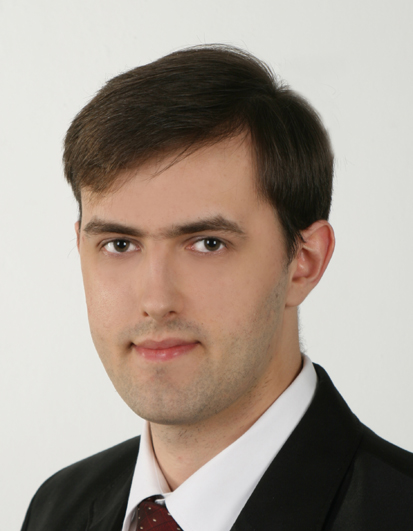
\includegraphics{my-photo.jpg}
%     }
%     \subfloat{
%     	%\begin{flushright}
%     		Kierunek: Informatyka
% 			\vspace{5mm} \\
% 	  		Specjalność: Inżynieria Systemów Informatycznych
% 			\vspace{5mm} \\
% 			Data rozpoczęcia studiów:	2013.10.01
%     	%\end{flushright}      
%     }      
% \end{figure}

\begin{minipage}[t]{0.3\textwidth}
% Pierwsza kolumna
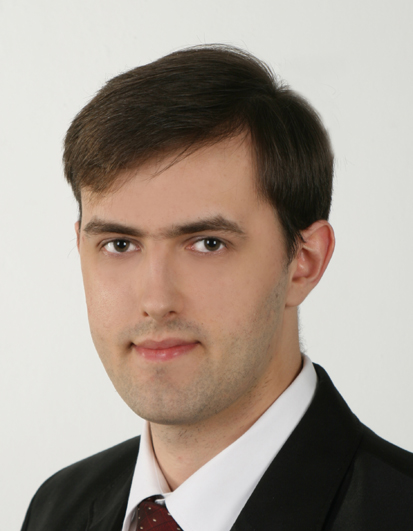
\includegraphics{my-photo.jpg}
\end{minipage}
\begin{minipage}[t]{0.7\textwidth}
\vspace{-45mm}
\emph{Kierunek:} \hspace{10mm} Informatyka
\vspace{5mm} \\
\emph{Specjalność:} \hspace{5mm} Inżynieria Systemów Informatycznych
\vspace{5mm} \\
\emph{Data rozpoczęcia studiów:} \hspace{5mm} 2013.10.01
\end{minipage}

\vspace{10mm} 

\begin{center}
\textbf{Życiorys}
\end{center}

Urodziłem się 7 stycznia 1990 roku w Warszawie. 
Ukończyłem I Liceum Ogólnokształcące im. Wacława Nałkowskiego w Wołominie.
W październiku 2009 roku rozpocząłem studia na Wydziale Elektroniki i Technik Informacyjnch Politechniki Warszawskiej na kierunku Informatyka. W czerwcu 2013 roku uzyskałem tytuł inżyniera. W marcu 2015 roku rozpocząłem roczne praktyki w CERN. 

% Urodziłem się 9 stycznia 1990 roku w Łodzi. W 1997 roku rozpocząłem edukację w Szkole Podstawowej nr 7 w Łodzi. W latach 2003-2006 kontynu- owałem naukę w Gimnazjum nr 42 im. Władysława Stanisława Reymonta w Łodzi. Od 2006 roku uczyłem się w Liceum Ogólnokształcącym nr 31 im. Ludwika Zamenhofa w Łodzi. W 2009 roku zdałem egzaminy maturalne i ukończyłem szkołę licealną z wyróżnieniem. W latach 2009-2013 studiowa- łem dziennie informatykę na Wydziale Elektroniki i Technik Informacyjnych Politechniki Warszawskiej. Ukończyłem studia z wynikiem celującym i ode- brałem tytuł zawodowy inżyniera. Obecnie kończę pracę dyplomową magi- sterską pod kierownictwem Instytutu Informatyki. We wrześniu 2012 roku rozpocząłem pracę zawodową jako programista aplikacji do zarządzania pro- cesami biznesowymi oraz aplikacji mobilnych w firmie Xentivo, gdzie pracuję do dziś. Moją pasją jest tworzenie aplikacji mobilnych oraz internetowych, które uruchamiane są w środowisku iOS.
	 
\begin{flushright}

\dots\dots\dots\dots\dots\dots\dots\dots\dots\dots\dots \\
    \fontsize{9pt}{9pt}\selectfont
      podpis studenta\hspace{18mm}\null
\end{flushright}

\begin{flushleft}
\begin{center}
\vspace{15mm}
\textbf{Egzamin dyplomowy}
\vspace{5mm} \\
\end{center}

Złożył egzamin dyplomowy w dn. \manydots	 
\vspace{5mm} \\
z wynikiem \manydots 	
\vspace{5mm} \\
Ogólny wynik studiów: \manydots	 
\vspace{5mm} \\
Dodatkowe wnioski i uwagi Komisji: \manydots	 
\manydots \\ 
\vspace{5mm}
\manydots
\end{flushleft}
	
\pagenumbering{gobble}


%!TEX root = thesis.tex
\newpage
\paragraph{Abstract} 
Transactions in non-relational databases, are a rare feature, but a useful and desirable one if present, such as Light Weight Transactions (\lwt) in the Cassandra.
The problem with \lwt is lack of a multi partition operations, which limits the practical applications, and puts the burden of maintaining the data consistency in other ways on the users.
The proposed multi-partition transactions algorithm removes the burden, supports transactions spanning many rows with read-committed isolation, and has a scalable design without a single point of failure.
We have achieved this by using \paxos algorithm for the distributed consensus, private memtables for isolation, and other techniques, which reduce memory footprint, and increase scalability.

% Multiple-inheritance hierarchies are data structures of a high importance in the area of
% the artificial intelligence. 
% The problem with them is lack of comprehensive and efficient methods of indexing, which
% limits the practical applications.
% The proposed hybrid indexing method can adapt to the particular topology of the data
% structure being processed. 
% We have achieved this by tuning the proportion between the member encoding methods to gain
% compactness of the index and fast responses of the search requests.
% Moreover, we have found that combining a few methods
% together preserves and even improves the ability to encode the changes incrementally.

% We have devised two member encoding methods: the first that bases on inheritance of some features and the second that
% bases on numbering schemes. The correctness of the developed solutions has been proved and their performance has been
% evaluated in the testing environment. The results show the characteristics of the hybrid index and prove its
% efficiency.

\paragraph{Keywords:} indexing transitive relations, multiple-inheritance hierarchy, reachability testing

\begin{center}
\vspace*{\baselineskip}
    \fontseries{b}\fontsize{15pt}{18pt}\selectfont
      Transakcje dla wielu partycji w Cassandrze  \\
\end{center}
\paragraph{Streszczenie} Hierarchie dziedziczenia wielokrotnego są strukturami danych o szczególnym znaczeniu w
obszarze zastosowań sztucznej inteligencji. Problemem, który ogranicza ich wykorzystanie w praktyce jest brak
uniwersalnej i efektywnej metody ich indeksowania. Zaproponowana hybrydowa metoda indeksowania dostosowuje się do
topologii przetwarzanej struktury danych. Osiągnięto to po przez dostrajanie proporcji pomiędzy składowymi metodami
kodowania, tak aby indeks był kompaktowy i oferował szybki dostęp do danych. Ponadto, połączenie komplementarnych metod
kodowania nie powoduje utraty zdolności do kodowania inkrementalnego, a nawet ją wspomaga.

% W ramach pracy stworzone zostały dwie składowe metody kodowania: jedna bazująca na dziedziczeniu cech, druga bazująca na
% schematach numerowania. Poprawność opracowanych rozwiązań została udowodniona, a wydajność sprawdzona w środowisku
% testowym. Wyniki obrazują charakterystykę hybrydowej metody indeksowania i dowodzą jej efektywności.

\paragraph{Słowa kluczowe:} indeksowanie relacji przechodnich, hierarchia dziedziczenia wielokrotnego, sprawdzanie
istnienia ścieżki w grafie

\pagenumbering{gobble}


\tableofcontents

% clearpage i pagenumbering resetują numerowanie stron
\clearpage
\pagenumbering{arabic}% Arabic page numbers (and reset to 1)



\chapter{Introduction}\label{chapter:introduction}

\section{Preface}\label{sec:introduction:preface}

\section{Motivation}\label{sec:introduction:motivation}

\subsection{Current state of transactions in Cassandra}	
Cassandra due to its distributed nature, cannot have full acid transactions, but it supports transactional behaviour with so called Lightweight Transactions (LWT).
LWT guarantees atomic modification of single partition iff specified condition is met. Main guarantee however is that after a successful LWT quorum of replicas agree on given value.

Conditions allow for example to do only insert if that row hasn’t existed before. 

Examples of LWT:

1)
INSERT INTO users (user_id, name, email)  VALUES (1, ‘John’, ‘john@yahoo.com’) IF NOT EXISTS

First example uses LWT to add user John with id=1 if John was not present in database. To put it differently, to insert a row to users table only if row with given key=1 didn’t exist.

2)
UPDATE balances SET balance = 2500 WHERE user_id = 1 IF balance = 2000;

Second example shows that conditions can have expressions that are evaluated during LWT. LWT will proceed further only if condition is met. Such expressions are restricted only to row that is being updated.

LWT is a tool which allows to have some consistency guarantees, but it is limited to single row. It cannot be used to have some transaction that spans two rows with conditions between them. 
To put LWT in terms of ACID, LWTs have serial isolation level, are atomic and durable. Consistency is preserved in terms of quorum, but not in terms of all nodes involved which is the case in relational world.

\section{Structure}\label{sec:introduction:structure}

%!TEX root = ../thesis.tex

\chapter{Theory}\label{chapter:theory}

\section{Distributed databases}\label{sec:theory:distDbs}
This section provides overview of non-relational distributed databases with main focus on the Apache Cassandra.

%Distributed databases are .. \ref{fig:hierarchyElements}. \cite{CassandraDataStaxDocs} \cite{chandra2007PaxosMadeLive} \cite{lamport1982byzantine}

\subsection{Cassandra}
% TODO referencje do Cassandry, krotki wstep o Cassandrze
% TODO wspomnieć o LWT.
Cassandra \cite{CassandraApacheDocs} \cite{CassandraDataStaxDocs} is a high performance, scalable, fault tolerant (i.e. no single point of failure), distributed post-relational database solution, which combines benefits of Google Bigtable \cite{chang2008bigtable} and Amazon Dynamo \cite{decandia2007dynamo}.
% to handle the types of database management needs that traditional RDBMS vendors cannot support. 

%Cassandra offers linear scale performance, which means that, for example if four nodes can handle hundred thousand 
%requests per second, then adding another four nodes results in the cluster, which can handle twice as much requests per second. Cassandra provides continous availability, due to redundancy of both data and node functions, which eliminate SPOF and provide constant uptime. 

\subsubsection{Key features}
Its key features are:
\begin{enumerate*}
\item masterless architecture,
\item linear scale performance \ref{sec:theory:cassandra:linear},
\item continuous availability,
\item flexible data model \ref{sec:theory:cassandra:datamodel},
\item multi data center support,
\item all nodes accept reads and writes,
\item Cassandra Query Language \ref{sec:theory:cassandra:cql}.
\end{enumerate*}

\subsubsection{Architecture}
Cassandra has a masterless \emph{ring} architecture \ref{fig:archCluster}, in which all nodes are equally significant, and there is no master node, therefore there is no single point of failure (SPOF). Cassandra uses replication, which is keeping copies of the data on multiple nodes, to also avoid SPOF during reads and writes. Cassandra provides continous availability, due to redundancy of both data and node functions, which eliminate SPOF and provide constant uptime.
Cassandra supports \emph{gossip} protocol, which is a scalable, distributed protocol used for inter-node communication.

\begin{figure}[h]
	\centering
	%\subfloat[The cluster on the ring]
	%{
	
\includegraphics[height=60mm]{images/cassandra-ring.png}\hspace{10mm}
	%}	
	\caption{A cluster on the ring}
	\label{fig:archCluster}
\end{figure}

\subsubsection{Replication}
Cassandra supports configurable replication via \emph{replication factor N}, which is the total number of nodes on which the data is stored, defined per \emph{keyspace} \ref{sec:theory:cassandra:datamodel}. A replication factor of $3$ means that three copies of the data exist across the cluster on $3$ different nodes.

Figure \ref{fig:replicationRing} shows a replication of the token $91$ in the cluster with $4$ nodes and the token ring with tokens ranging from $0$ to $99$. 
Each node is the \emph{primary replica} for the token range placed counter clock-wise to it, thus node $1$ is the primary replica for range $75-0$, node $2$ for $1-25$, node $3$ for $26-50$, and node $4$ for $51-75$. 
Token value $91$ belongs to the node $1$, and since $N=3$, then the value is replicated on $2$ more nodes, which are on counter wise positions, thus on node $2$ and node $3$, which are \emph{secondary replicas} of the token. 

% źródło https://pandaforme.gitbooks.io/introduction-to-cassandra/content/understand_replication.html
% prawdziwe źródło to prawdopodobnie kurs z DataStax, ale nie mogę tego znaleźć.
\begin{figure}[h]
	\centering
	%\subfloat[The cluster on the ring]
	%{
	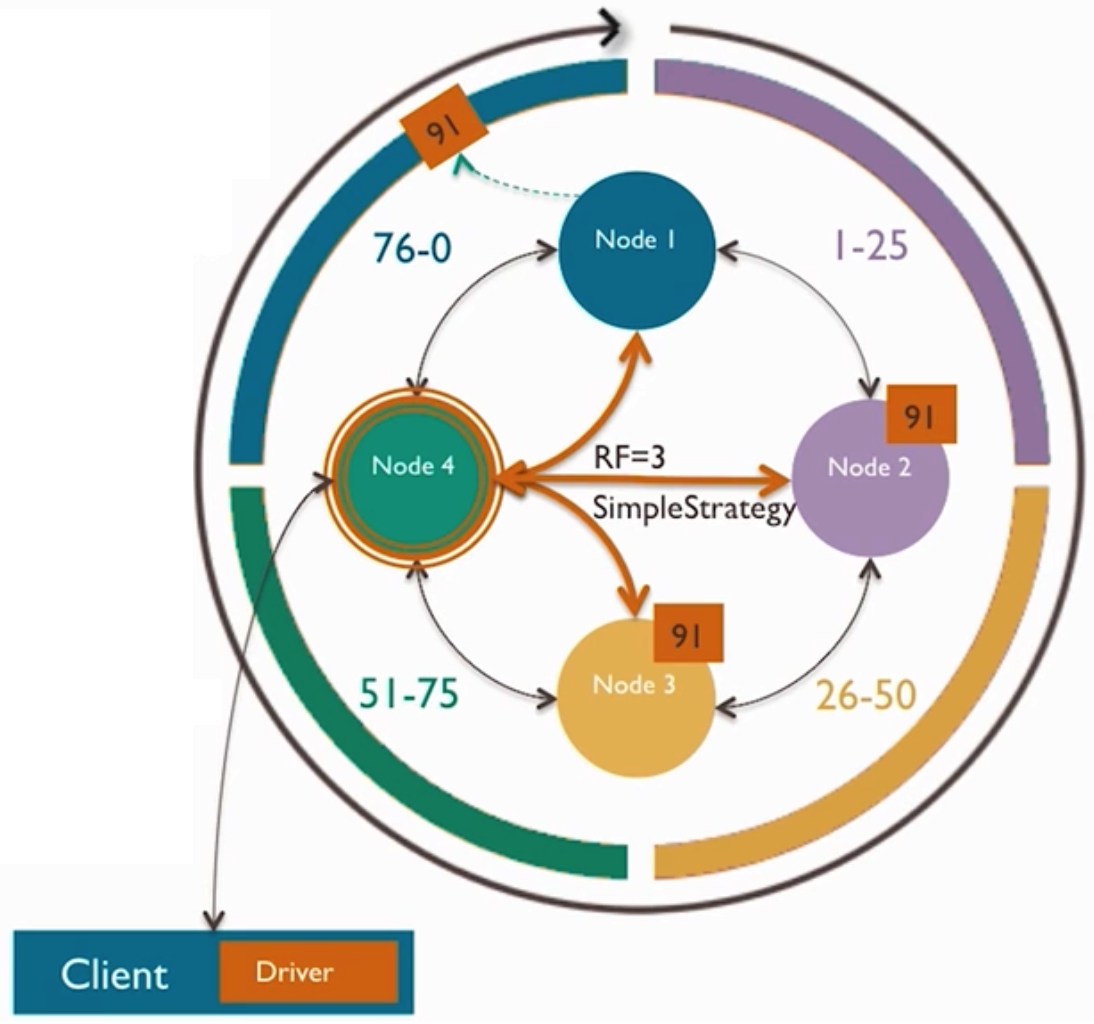
\includegraphics[height=100mm]{images/cassandra-replication-ring.png}\hspace{10mm}
	%}
	%\label{fig:replicationRing}
	\caption{Replication of the token 91}
	\label{fig:replicationRing}
\end{figure}

%\subsubsection{Read path}
%TODO Read path
%\subsubsection{Write path}
%TODO Write path

%Architecture
% Token ring
% rysunek z klastrem



\subsubsection{Data model}
\label{sec:theory:cassandra:datamodel}
Cassandra's data model is a wide-row store, which consists of tables, which reside in keyspaces\footnote{comparable to schemas in RDBMS} with rows, identified by primary keys, with up to 2 billion columns. Although data model concepts are similar to relational ones, data modeling techniques depart from the relational modeling, since models are supposed to be highly denormalized, which provide ability to perform fast queries by reading a single partition, which is the unit of the data replication in Cassandra, in order to fetch all the data the query needs without further communication with other nodes and performing joins\footnote{which do not exist in Cassandra}.

%\begin{description}
%\item[keyspace] 
%\item[table]
%\item[column]
%\item[row]
%\item[primary key]
%\end{description}

\subsubsection{Linear scale performance}
\label{sec:theory:cassandra:linear}
Cassandra offers linear scale performance, which means that if two nodes can handle hundred thousand requests per second, then adding another two nodes results in the cluster, which can handle twice as much requests per second. Figure \ref{fig:archLinearScale} depicts the example.

The key principles behind linear scaling are:  data partitioning and token ranges. 
Partitioning is the assignment of the token values, which are \emph{long} values, to the keys, and more concretely to the partitioning keys of a primary key. Cassandra provides different \emph{Partitioners}, which implement different algorithms to perform such token assignment. \emph{Murmur3Partitioner} uses \emph{Murmur3} hash algorithm that provides a good distribution over the hash space, and is fast due to the fact that it does not support cryptographic properties, which are not required by Cassandra.

Each node is responsible for a token range, which is a part of the token ring. Responsibility means that a node stores the data for which the token value falls into its token range. When a new node is added, it automatically receives a token range and then the data is moved between the nodes in order to adjust to the new division of the token ring.

Correct data modeling is also an important aspect of the linear scalability, since partitioning keys of tables have to be designed in a way that provides high cardinality of the keys. Otherwise part of the cluster starts to collect more data than its storage capabilities, and it will fail. 


\begin{figure}[H]
  \centering  
  % TODO źródło?
  % Źródło http://docs.datastax.com/en/cassandra/2.1/cassandra/images/intro_cassandra.png
  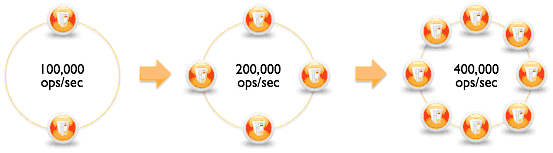
\includegraphics[width=\textwidth]{images/cassandra-linear-scalability.png}\hspace{10mm}  
  \caption{The linear scalability from 100k to 200k requests per second}
  \label{fig:archLinearScale}
\end{figure}


%Linear scale performance is provided by even assignment of token ranges of the token ring to the nodes in the cluster combined with data \emph{partitioning} -- which is assigning a token values to the keys -- that evenly distributes the data around the cluster. When a new node is added to the cluster, it automatically 


\subsubsection{Cassandra Query Language}
\label{sec:theory:cassandra:cql}
Cassandra Query Language (CQL) is the query language, similar in syntax to SQL, but provides only limited functionality compared to SQL, as there are no joins, inner queries, nor aggregations. CQL provides select, insert, update and delete statements. Select statement's \emph{where} clause supports equality condition on the partition key columns and restrictions such as: IN, =, >, >=, <= and < on the clustering columns. Columns, which are not part of the primary key cannot be restricted in the \emph{where} clause. Listing \ref{lst:cqlSelect} shows two examples of select statements, first with equality restriction on the partition key column \emph{user_id}, second with equality restrictions on the partition key columns: \emph{cluster}, \emph{date}, \emph{datacenter}, and range restrictions on the clustering key columns: \emph{hour} and \emph{minute}.
%Cassandra uses binary protocol named Cassandra Query Language (CQL). In order to do anything with database, we need to use a driver that speaks binary protocol. 

\begin{lstlisting}[style=outcode,label={lst:cqlSelect},caption={Examples of CQL select statements}]
SELECT user_name, user_email 
FROM app.users 
WHERE user_id = 10123;
    
SELECT * FROM app.requests
 WHERE cluster = 'cluster1'
 AND date = '2015/06/05'
 AND datacenter = 'EU_NORTH'
 AND (hour, minute) >= (12, 0) AND (hour, minute) <= (15, 30);
\end{lstlisting}

 
\subsubsection{Use cases}
Cassandra is a general purpose non-relational database, however there are areas in which Cassandra excels over other databases:
\begin{enumerate*}
\item internet of things applications - Cassandra is able to consume large quantity of incoming data\footnote{depends on cluster size} from devices, sensors and similar internet connected devices,
%\item E-commerce - durable shopping cart protection combined with fast product catalog browsing
%\item Messaging - Cassandra serves as the database for mobile phone applications
\item data analytics - Cassandra provides storage with fast access to the data for analysis. Apache Spark, which is an engine to perform large-scale data processing \cite{ApacheSpark} supports Cassandra, as one of its data sources, therefore Cassandra provides data storage for analytics and also stores results of the analysis done in Spark,
\item storage of time series data - Cassandra's fast writes, wide-rows and ability to read only particular data ranges are well suited for time series based applications, because such data fits natively into the data model.
\end{enumerate*} 

\subsubsection{Transactions}
Cassandra does not provide ACID compliant transactions, but it offers Light Weight Transactions, which offer a degree of transactionality limited to the scope of single partition, therefore to the single primary key\footnote{concretely to the partitioning part of the key in terms of the complex key}. Section \ref{sec:theory:transactions:lwt} provides more on this subject in comparison to other distributed transactions. 

\subsubsection{Compared to RDBMS}
\begin{figure}[hbt]
  %\centering
  \setlength{\unitlength}{1.3cm}  
  \subfloat{
    \renewcommand{\tabcolsep}{0.1cm}
    \resizebox{\textwidth}{!}{\begin{tabular}{c|c}
      \toprule
      RDBMS & Cassandra  \\ \midrule
      manages structured data      &  manages any type of data    \\
      ACID transactions 		   &  simple transactions supported by LWT \\
      SQL & CQL \\
      scales vertically & scales horizontally \\
      master-slave architecture & masterless, share nothing architecture \\
      denormalization is the bad practice & denormalization is the best practice \\
      single points of failure with failover & no single points of failure \\  \bottomrule      
    \end{tabular}}
  }
  \caption{RDBMS compared to Cassandra}
  \label{fig:cassandraToRdbms}
\end{figure}

\subsubsection{Eventual consistency}\label{sec:theory:eventualConsistency}
In terms of CAP \cite{brewer2000towards} \cite{Brewer:2012ba} Cassandra is the \emph{AP} database with eventual consistency, which means that over time the data becomes consistent on all nodes, but there are no guarantees about the time it takes. Cassandra uses techniques such as: \begin{enumerate*} 
\item \emph{hinted handoff} - stores a message for the currently unavailable replica about the modification and sends it to the replica when it comes back up \cite{CassandraHintedHandoff},  
\item \emph{read repairs} - detects inconsistency in the data during read and repairs it by sending a message with the data \cite{CassandraReadRepair},  \end{enumerate*} to pro-actively reduce incosistency in the data during normal operations.

\subsection{MarkLogic}
MarkLogic is a NoSql database with the document-centric schema-agnostic data model \cite{markLogicDataModel} with native support for formats such as JSON, XML and RDF, and support of ACID transactions \cite{markLogicAcid}.

ACID transactions are implemented by the means of multi-version concurrency control (MVCC) and locking. In an MVCC system, changes are tracked with a timestamp number on each document. 
The database uses these timestamps to ensure that all users see consistent data. 
Transaction has to acquire write locks on all of the updated documents and read locks on all of the queried documents in order to complete evaluation. Acquired locks are held until the transaction ends, which prevents other transactions from updating the read locked documents and ensures a read-consistent view of the documents. 
Deadlocks might happen, but are detected by the database, and are dealt with by aborting one or the other request and retrying it later \cite{markLogicUnderstandingTransactions}.

% Bazy które wspierają jakieś transakcje
% ACID transactions

\subsection{FoundationDB}
FoundationDB is a NoSql database with ACID compliant transactions, strong scalability and SQL querying capabilities.
Its core data model is a ordered key-value store, in which the ordering property increases efficiency of range reads. It also supports document store and relational DBMS as layers on top of the core model. 

FoundationDB was acquired by Apple \cite{foundationDbAcquired} and since then no information is available. Its website is shutdown, documentation is not accessible nor downloads of the database. According to the press, the database scaled up to $14,4$ million random writes per second.
% Było, miało transakcje, zostało wchłonięte przez Apple i znikneło z Internetu

% TODO inne rozproszone bazy z transakcjami, takie jak Cassandra

\subsection{Distributed relational databases}
Distributed Relational Database Architecture (DRDA) \cite{drda} is an open standard architecture for distributed relational databases, which provide relational data, but distributed among multiple platforms, which communicate with each other. An example of a DRDA compliant database is the DB2 created by IBM. The database supports SQL queries, which can access tables from different platforms. 

Since there are only few DRDA databases existing mostly around IBM ecosystem and since there are many distributed NoSql databases, which gain on popularity, then the conclusion is that distributed relational databases are not the right solution to the problem of big data.

\section{Transactions}\label{sec:theory:transactions}
Transactions in RDBMS

% TODO organizacja rozdziału, czy paxos powinien mieć pełny opis, czy tylko referencja? 
\subsection{ACID}
TODO Czy ja w ogóle powinienem to rozszerzac? Czytelnik powinien to znac.
Transactions in relational databases are ACID compliant, which means that a transaction is \begin{enumerate*} 
\item Atomic - either all statements in the transaction succeed or none,
\item Consistent - TODO
\item Isolated - transactions do not interfere with each other during execution,
\item Durable - changes made by a committed transaction are preserved even after the database failure.
\end{enumerate*}

\subsection{2 phase commit}

\section{Distributed transactions}
% TODO rozrysować co czym jest, Raft, Paxos -> distributed consensous algorithm
% RAMP atomic commit

% LWT (CAS) distributed transaction, compare and set with distributed consensous. Implementacja w Cassandrze.

\subsection{3 phase commit}\label{sec:theory:transactions:3pc}

\subsection{Paxos}

since it has network partition tolerance, it has advantage over \emph{3PC} (\ref{sec:theory:transactions:3pc}).

% TODO opisać na tyle szczegółowo żeby móc je porównać. 
% bez dokładnego schematu
% ogólny schemat, najbardziej typowy przypadek opisać, bez dowodów, bez wyników testów.
% żeby było wiadomo o co chodzi.

% po to żeby móc porównać, Paxos jest lepszy od 3PC bo (ma partycje) i źródło "dokładnie jest to opisane tu i tam"
% ma wynikać z jakiego powodu jest lepszy


%  Paxos, Raft, 3PC opisane na jednym poziomie szczegółowości

% żeby do zrozumienia pracy nie trzeba było zaglądać gdzieś indziej.


\subsection{Raft}
% TODO napisać jakie to są guarantees
\emph{Raft} algorithm offers the same guarantees, as \paxos. 
The aim of Raft designers was to create a consensus algorithm which would be more understandable to its predecessor \cite{ongaro2014search}. 
The main idea behind the algorithm is decomposition of the consensus problem into the following individual tasks:
\begin{enumerate*}
\item leader election,
\item log replication,
\item safety,
\item membership changes.
\end{enumerate*} 
%Safety property is that: if any server
%has applied a particular log entry to its state machine,
%then no other server may apply a different command for the same log index.
 A server supporting \emph{Raft} is in one of three states: \begin{enumerate*} \item leader, \item follower, \item candidate \end{enumerate*}. The leader can be only one and it handles all client requests. When a follower receives a request, it has to redirect request to the leader. The candidate state is used during leader election. 
% TODO reszta opisu

 %The difference to \paxos  is that \emph{Raft} has been decomposed into independent subproblems which clearly address problems. 

% TODO %
% Napisać jak ten RAFT działa
\emph{Raft} uses \emph{Leader election}. Leader is elected for specific term. \emph{Raft} uses \emph{Log Replication} to arrive at consensus. Leader proposes new value to \emph{followers} which append value to uncommitted log. Once leader has majority of acknowledges it sends commit message. Followers receive commit message and commit value in the log. 

\emph{Raft} algorithm is visualized in \cite{raftVisual}.

\subsection{RAMP}\label{sec:theory:transactions:ramp}
\emph{Read Atomic Multi Partition} transactions \cite{Bailis:2014} is the newest algorithm among the algorithms discussed in this chapter. 
\emph{RAMP} algorithm was designed to address the requirements of the following use cases: secondary indexing, foreign key
enforcement, and materialized view maintenance.
\emph{RAMP} identifies new transaction isolation level \emph{Read Atomic}, which 
assures consistent visibility of changes made by the transaction: either all or none of each transaction's updates are seen by other transactions.
\emph{RAMP} is resilient to partial failures -- failures of part of the nodes in the cluster -- for the reason that RAMP's transaction does not contact nodes that are not affected by the transaction. 
\emph{RAMP} also guarantees \emph{synchronization independence}, which means that transactions do not stall or fail other transactions, due to the fact that reads and writes do not block each other. 

%The transaction is able to detect non-atomic partial read and repair it with additional rounds of communication with nodes. 
The key principle behind \emph{RAMP} is its ability to detect non-atomic partial read, and to repair it with additional rounds of communication with the nodes by the means of \emph{the metadata} attached to each write and \emph{multi-versioning}, which means that the data is accessible in different versions and each modification to the data creates a new version. Versions are either committed or not yet committed, in which case the data can be discarded by aborting the transaction \cite[p. 6]{Bailis:2014}. 
There are three variants of \emph{RAMP} algorithm and the difference between them is the type of the metadata. \emph{RAMP-small} uses a 64 bit timestamp as the metadata and requires additional two rounds of communication when non-atomic read is detected. Other variants of \emph{RAMP} are described in \cite[p. 5]{Bailis:2014}.
\emph{RAMP} was proven to be linearly scalable with the number of nodes during trials spanning up to 100 servers \cite[p. 10]{Bailis:2014}.

%  TODO Może to gdzieś się opłaca dodać:
% \emph{RAMP} transactions (\ref{sec:theory:transactions:ramp}) have support for multi-partition operations. 
% However \emph{RAMP} relies on 64 bit timestamp \cite[p. 8]{Bailis:2014} which is not the current standard \cite{timestamp64wiki}, thus \emph{RAMP} cannot be used at the time being.
%

\subsection{LWT}\label{sec:theory:transactions:lwt}
% TODO źródło w (more on this)
As mentioned earlier, Light Weight Transactions is the name of compare-and-swap functionality implemented in Cassandra. Internally, LWT uses the Paxos algorithm with some modifications which were aimed to prevent potential single point of failure, thus improving high availability. SPOFs may surface in case the leader fails when it is about to propose a new value (more on this…). The problem was addressed by sacrificing the standard leader election in favour of allowing any node to act as a leader, so that it can propose a value at any time. On the downside, such approach increases the risk of contention. 

One of the key requirements of Paxos protocol is storage of PaxosState - a data structure composed of the proposed value, proposed ballot, promised ballot and most recent commit. In case of LWT, the value represents the update itself along with the token of the partition key where that update should be applied. That token uniquely identifies PaxosState so that several proposals for the same partition can be associated with the same Paxos instance. 


LWT includes the following phases: \begin{enumerate*}
\item prepare,
\item get promise,
\item read row,
\item get results,
\item propose a new value,
\item acceptance,
\item broadcast commit,
\item wait for acknowledgements.
\end{enumerate*} Let us analyze each of them in the environment with 5 nodes, replication factor 3 and request to insert user named \emph{John} to \emph{users} table, but only if \emph{John} does not exist. For simplicity, \emph{users} table has only two columns: \begin{enumerate*} 
\item name -- text column and primary key, \item email -- text column. \end{enumerate*} LWT begins with a node 5 receiving request. Node 5 is then called coordinator node. The coordinator has to become the leader of paxos round identified by the token computed from partition key of \emph{users} table, thus from string value \emph{John}. To become the leader, the coordinator has to create the new ballot and send it along with the token and table name to replica nodes: node 1, node 2, node 3. Each replica has to check whether the ballot is the highest ballot it has seen, and if it is, then replica saves it in the PaxosState and responds with a promise. The leader has to wait for majority of promises before it proceeds. When majority promises, the coordinator may proceed to read the row and check the condition. The condition is that \emph{John} cannot exist, thus read has to not find any rows querying users by user name \emph{John}. Let us assume that indeed user \emph{John} did not exist, thus condition is met which allows the coordinator to propose an insert of \emph{John} with email \emph{john.doe@gmail.com} to \emph{users} table. The coordinator sends proposal message, with an insert and same ballot, to replicas and waits for acceptances. A replica saves proposed insert to PaxosState and replies with acceptance message.
When the coordinator receives majority of acceptances it broadcasts the commit message and waits for majority of acknowledgements. Upon receiving commit message a replica applies an update stored in PaxosState, thus it performs the insert of \emph{John} to \emph{users} table and acknowledges commit with a reply.

At any time during whole procedure the minority of replicas might stop responding and LWT can continue. In case of the example, one node can fail without aborting \emph{LWT}. If more than one node fails, then LWT is aborted. 

Secondly, at any time the leader might lose leadership if a other node does prepare with a higher ballot. In that case the coordinator has to wait, giving the other leader time to complete its \lwt, and try again with new ballot.

Note that \lwt affects only limited number of nodes -- replicas of the key, thus majority is considered only at the level of replicas, not at the level of the cluster.


%1. LWT is initiated by client request: insert John if not exists
%2. Request is routed to some node X that becomes coordinator of LWT
%3. Coordinator wants to be a leader so it creates a ballot and sends prepare to replicas: node1, node2, node3. This is prepare phase.
%4. Replicas promise to not accept values from leaders who have lower ballots.
%5. Coordinator gets 3 of out 3 promises. Quorum promised to listen.
%6. Coordinator performs read: SELECT * FROM users WHERE user_id = 1
%7. Coordinator checks condition “IF NOT EXISTS”. If such row did not exist in quorum of replicas it proceeds further
%8. Coordinator, as a leader, proposes new value which is an insert to users table.
%9. All three nodes reply with accept. Quorum accepted insert.
%10. At this point, insert is an in progress proposal that has been accepted by majority of replicas. Even if coordinator crashes, once someone selects user with id=1 or retries to insert it. This proposal will get committed. Let’s assume that coordinator is well and proceeds to commit.
%11. Coordinator broadcasts commit message
%12. Replicas apply insert locally and reply with acknowledge message
%13. Coordinator receives quorum of acknowledges. LWT has been successfully completed.
%14. Coordinator responds to client: John was inserted.


%Sequence above is a happy path. At any point coordinator might lose his leadership if some other node sends prepare with higher ballot. In that case coordinator waits a bit and retries whole process again. 
%Also any replica might stop responding, which is fine as long as quorum is up and well. If quorum responds to messages, coordinator can proceed. If there is no quorum then paxos conditions are not met and LWT cannot be continue. However during normal operation is it rather rare to see many nodes down so in general LWT can successfully finish with 2 out of 3 replicas running. Note that cluster size might be much bigger, for example hundred nodes, but since replication factor N=3, only three nodes are interesting from perspective of LWT and Paxos.


\subsection{Datomic}
% TODO podejście na jeszcze wyższym poziomie abstrakcji. 


%!TEX root = ../thesis.tex

\chapter{Multi partition transactions algorithm}\label{chapter:mpp}

Multi partition transactions algorithm (\mpt) uses \paxos, and leverages the distributed consensus with other techniques presented in this chapter to provide multi partition transactions with read-committed isolation level.

%!TEX root = ../thesis.tex

\section{The rationale}
The \mpt algorithm is designed for distributed databases with token ring architecture,
which uses \emph{keys} to lookup replicated data in the cluster. Its key features are: \begin{enumerate*}
\item supports multi-partition operations,
\item supports transactions with read-committed isolation level,
\item supports transactions that are atomic and durable,
\item is resilient to network partitions. In terms of \emph{CAP} \cite{Brewer:2012ba} it uses \emph{AP}.
\end{enumerate*}


%!TEX root = ../thesis.tex

\section{The algebra}
Database consists of key-value pairs $\Omega((k_{i},v_{j}), (k_{k},v_{m}),...)$ where $k\in\mathit{K}, v\in\mathit{V}$ stored by cluster of nodes $\mathit{N}$. Node is defined, as $n_{i}\in\mathit{N}$ where $\mathit{N}$. Client of a cluster is an actor, which communicates to a cluster, denoted by $c_{i}\in\mathit{C}$. Changes to data are represented by \emph{mutations}, where mutation is defined by $\delta(k,v)$ where $k \in \mathit{K}, v \in \mathit{V}$.
A set of mutations is a transaction denoted, as $\Theta(\delta_{1}, \delta_{2}, ...)$. Topology is a partitioning function $\tau:\mathit{K} \mapsto \mathit{N^{RF}}$ which given $k$ returns set of replica nodes. 

\emph{Transaction state} is defined by $\Lambda(\lambda_{i}, \lambda_{j}, ...)$ where $\lambda_{i}$ is \emph{transaction item}, which is equivalent\footnote{transaction item is redefined in Chapter 4} of a key $k$.

\section{The outline}
Database consists of key-value pairs $\Omega((k_{i},v_{j}), (k_{k},v_{m}),...)$ where $k\in\mathit{K}, v\in\mathit{V}$ stored by cluster of nodes $\mathit{N}$ in which a node is defined, as $n_{i}\in\mathit{N}$.
Changes to data are represented by \emph{mutations}, where mutation is defined by $\delta(k,v)$ where $k \in \mathit{K}, v \in \mathit{V}$. Transaction is set of mutations denoted, as $\Delta(\delta_{1}, \delta_{2}, ...)$.

Client denoted, as $c_{i}\in\mathit{C}$ is an actor, which performs transactions $\Delta_{1}, \Delta_{2}, ...$ and communicates to \nodes via messages $\mathit{M}$ (Definition \ref{def:message}).

%\nodes expresses number of nodes and \node{i} refers to a node, where $i \in [1,N]$.

 \client begins a transaction \transaction by sending a request to any node in a cluster \clientReq{i} and receives response \nodeReqResponse{i}, which includes 
initial \emph{transaction state}, which reflects all changes done in \transaction and is defined as \emph{transaction id} and set of \emph{transaction items}. Transaction id identifies the transaction and is attached to all subsequent requests. 

%Transaction id identifies the transaction and is attached to all subsequent requests. Transaction item is a reference to operations done in \transaction.

Client \client performs two types of operations during \transaction: \emph{mutations} \mutations, as in Definition \ref{def:mutation} and select statements of \kv. All \mutation{k}{v}  performed by \client are isolated from other clients and are private to \transaction until \transaction is committed. Mutations are stored in a \emph{private transaction storage}, which is a local data structure at each \node{i}, for the duration of the transaction, whereas read operations query against current state of the database, thus transactions provide read-committed isolation level.

After each \clientReq{i} with a \mutation{k}{v} \client receives a response \nodeReqResponse{i}, which includes a transaction item referencing the \mutation{k}{v}. Client is responsible for tracing changes performed in \transaction, thus \client has to append all received transaction items to the initial transaction state.

When \client finishes its planned operations \transaction can be either committed or rolled back. To perform rollback \client performs \clientReq{i} including transaction state, and then \node{i} sends out rollback messages to other nodes \nodeMessage{i}{j,k,l,...}, identified using transaction items, which remove private data from their private transaction storage and mark \transaction as rolled back in \emph{transaction log}, which is a local data structure.

In order to commit \transaction \client performs \clientReq{i} with transaction state attached, and subsequently \node{i} becomes the coordinator of the transaction and is responsible for orchestrating distributed consensus among nodes affected by \transaction referenced by transaction items. When consensus is reached each node moves private data of \transaction from private transaction storage to the main storage and marks \transaction, as committed in transaction log. Client receives response \nodeReqResponse{i} about successfully committed transaction.

There are many concurrent transactions and some of them mutate same keys, thus concurrency control is required which gurantees that interfering transactions are not committed at the same time. Commit procedure solves this problem by grouping such transactions and performing distributed consensus round, which selects single transaction that is committed, whereas the rest is rolled back.
Commit procedure uses another local data structure \emph{transaction index}, which is responsible for identifing interfering transactions and grouping them into same consenus rounds.

\begin{definition}
  \label{def:mutation}
  \emph{Mutation} denoted as \mutation{k}{v} is an operation, such as insert, update or removal of one or more key value pairs \kv.
\end{definition}

\begin{definition}
	\label{def:message}
	\emph{Message} is defined by $\mathit{M}(n_{i}, n_{j}, \psi)$ where $n_{i}\in\mathit{N}\cup\mathit{C}, n_{j}\in\mathit{N}\cup\mathit{C},\{n_{i}, n_{j}\}\cap\mathit{N}\neq\emptyset$.
	$n_{i}$ is sender of a message, $n_{j}$ is recipient of a message, $\psi$ is a payload, which is one of following: \\	
	$\mathit{begin\_transaction}()$ -- begins transaction \transaction \\
	$\mathit{initial\_transaction\_state(\sigma)}$ -- message in response to $\mathit{begin\_transaction}$ message where $\sigma$ is initial \emph{transaction state} (Definition \ref{def:transactionState}) \\
	$\mathit{select(k)}$ -- is a selection of the value corresponding to $k$ \\
	$\mathit{data(k,v)}$ -- is a message in response to $\mathit(select(k)$, where $v\in\mathit{V}$ \\
	$\mathit{insert(k,v)}$ -- is an insert of key-value pair \\
	$\mathit{update(k,v)}$ -- is an update of key-value pair \\
	$\mathit{delete{k}}$ -- is a delete of value associated with key \\
	$\mathit{transaction\_commit(\Lambda)}$ -- is a commit of a \transaction, where $\Lambda$ is final transaction state \\
	$\mathit{setup(\Lambda)}$ -- inititates \emph{setup phase} of \mpt algorithm \\
	$\mathit{prepare(\Lambda, \beta)}$ -- initates \emph{prepare phase} of \mpt algorithm; $\Lambda$ is final transaction state, $\beta$ is \paxos ballot \\
	$\mathit{promise(promised, log, inProgress_{\Lambda})}$ -- is a response to $\mathit{prepare}$ message, where $\mathit{promised}$ is a boolean, $\mathit{log}$ is state of \emph{transaction log} \ref{sec:mpp:transactionLog}, $\mathit{inProgress_{\Lambda}}$ is accepted but not yet committed transaction state \\
	$\mathit{propose(\Lambda, \beta)}$ -- initates \emph{propose phase} of \mpt algorithm
	$\mathit{propose\_response(accepted, log)}$ -- is a response to $\mathit{propose}$, where $\mathit{accepted}$ is boolean, $\mathit{log}$ is state of transaction log \\
	$\mathit{commit(\Lambda)}$ -- initates \emph{commit phase} of \mpt algorithm, where $\Lambda$ is transaction state \\
	$\mathit{commit_ack()}$ -- is an acknowledge of $\mathit{commit}$ message \\
	$\mathit{update\_transaction\_state(\lambda)}$ -- is a message in response to $\mathit{insert, update, delete}$ messages where $\lambda$ is transaction item (Definition \ref{def:transactionItem}) 
\end{definition}


\subsection{Brudnopis z oznaczeniami}

Node denoted as $n_i$ where $i \in $


Nowe oznaczenia:

$\sigma$ transaction state

Clients and nodes communicate by messages, where message is defined, as $\mathit{M}(n_{i}, n_{j}, \psi)$ where 
$n_{i}\in\mathit{N}\cup\mathit{C}, n_{j}\in\mathit{N}\cup\mathit{C},\{n_{i}, n_{j}\}\cap\mathit{N}\neq\emptyset$ and $\psi$ is a payload, which is one of following:
- $\mathit{begin\_transaction}()$
- $\mathit{begin\_transaction_response}(\sigma)$
- begin transaction response(ts)
- insert(k,v)
- insert response()
- update(k,v)
- delete(k)
- commit(ts)
- setup(ts)
- prepare(ts, b)
- propose(ts, b)
- commit(ts)


Client request \clientReq{2}

Node response \nodeReqResponse{2}

Node message \nodeMessage{1}{2}

Node response message \nodeMessage{2}{1}

Key \key

Key i \keyi{2}

value \kvalue

value i \kvaluei{3}

key value \kv

Mutation \mutation{k}{v}

TODO poprawa oznaczen
Transakcja to zbiór mutacji (male delty)

3 rozdział brak tokenów, brak tabeli

tokeny i tabele dopiero w implementacji.  - rozdzial 4

Rozdzial 3 najbardziej ogólnie, nic o Cassandrze.

Rozdział 4 jak to zostało zaimplementowane dla Cassandry.

Zamiast request response zdefiniować message który dzieli się na typy.
message ma źródło, cel, payload. Payloady to rozne typy

Funkcja noda to f: M -> M 
czyli funkcja ktora przeklsztalca message w message. 
Dzialanie noda jest zdefiniowane przez funkcje jaks tam bo zawsze masz request response.
f: (S, M) -> (S, M)
gdzie S to stan noda.

2.3.2 uprościć o CAP

2.2
Poprzec literaturą stwierdzenia, że RDMBS ma ACID, a NoSql nie ma.

Przedstawiać bazy relacyjne i bazy nierelacyjne
Bazy rozproszone i bazy nierozproszone.

Nie mówić o bazach relacyjnych i bazach rozproszonych

Paxos
Coordinator node Propser
Node 1,2,3 Acceptor

Figure 2.3 Paxos pokazać przypadek z drugim proposerem.

2PC, 3PC, Paxos przedstawiane z różnej perspektywy.
Porównać w każdym przypadku odporność na awarie.

Wyodrębnić zbiór aspektów który będę porównywał. 
Akapit per aspekt tak żebym móc porównać jeden z drugim.

Cechy specyficzne w pierwszym akapicie.

1 Co to jest, cechy specyficzne
2. akaip to ogólny Opis
3. Aspekt 1
4. Aspekt 2
5. Aspekt 3




%!TEX root = ../thesis.tex

\section{Multiple partitions}\label{sec:mpp:requirements}
%TODO Note: tytul zmieniony z The requirements na Multiple partitions
% TODO rozwinąć wymagania na algorytm, wykrywanie instacji. Z tego przejść do wymagań Paxosa. Następnien pisać na jakich wymaganiach trzeba się skupić, bo one nie będą proste do spełnienia.


% TODO wspomnieć o tym, że LWT używa wielu instacji paxosa które ze sobą nie kolidują bo dotyczą różnych partycji, a u mnie jest inaczej ponieważ transakcja może dotyczyć wiele partycji i dodatkowo mogą się pokrywać.
% TODO w LWT żeby poznać instacje paxosa  wystarczy klucz partycji.
% TODO MPP jest to problem bo jest wiele partycji
\lwt supports many instances of paxos protocol at any given time, which do not interfere with each other, unless the same partition keys are considered. \lwt instances for different keys do not overlap nor stall each other.
\mpt supports many instances as well, but a single instance of \mpt might overlap with different instance of \mpt, in which case such instances are considered conflicting. 

\lwt identifies \emph{paxos round} by a partition key. The key difference to \lwt is that \mpt instance is associated with many keys, thus instance of \mpt cannot be identified by a partition key. 
Distinction between \paxos rounds in \mpt is troublesome because it is not obvious how to reflect a set of different keys as a single round identifier.
\label{sec:mpp:requirements:identifyRound}

\lwt is for a single partition, therefore it represents a single operation. As such, operation itself is a \emph{transaction}. Data for that transaction is passed within operation itself, thus data does not have to be stored for the duration of the transaction, because it exists only in memory while \lwt transaction executes. 
On the other hand, \mpt supports many operations within a transaction. Therefore operations with data have to be stored for the duration of the transaction. Moreover, storage has to be private for the transaction in order to provide isolation.

%Proposed \mpt holds all imposed requirements. Following sections address requirements in context of \mpt.

%Transactions should have following functionality:

%TODO napisac czym sie roznica od LWT - dodatki do prywatne dane - to juz opisalem w The advantage \\
%TODO napisac czym sa memtable - tylko pytanie gdzie to napisac, to moze byc opisane w innej sekcji \\


%1. Run in isolation from other transactions - transactions - their state and data - should be isolated from each other. One transaction cannot see other’s data.
%2. Serializability - if two transactions modify same piece of data and commit at same time, only one transaction can be committed, as a corollary second has to be rolled back.
%3. Begin transaction - that how any transaction is started in relational databases. Transaction is begun and then 
%4. Commit transaction - once transaction’s logic has finished, user commits transaction and sees either successful commit or rollback of transaction. 
%5. Rollback transaction - rollback whole transaction if needed
%6. Do an operation within transaction - any data manipulation operation should be possible to execute in context of transaction
%7. Atomicity
%8. Durability
%9. Eventual consistency


%        Requirements summary
%All of requirements above were addressed in algorithm. There is an solution to each requirement in next sections followed by summary of whole algorithm.




%!TEX root = ../thesis.tex

\section{Representation of transaction}
Transaction state has \emph{unique id} (UUID\footnote{universally unique identifier}) along with all operations and data done within transaction, thus all modifications. 
Each modification is performed for one key. Key belongs to a partition, thus modification is performed for single partition. There can be many modifications done within transaction. 

\subsection{Tokens}
Each key has a token which belongs to the token ring. Token for key is computed by hash function. \mpp is not dependent on concrete hash function. Tokens are numbers. In case of \emph{JVM} tokens are of type \emph{long} which occupies 8 bytes of memory. Keys are not restricted by any type, thus key can be a 100 character long string which requires around $232$ bytes\footnote{concrete size depends on \emph{JVM} options used}. Size of the key is then 29 times size of a token. Complex keys can have even bigger size. Token is deterministic in size and in most cases occupies less memory than key itself.

Ranges of token ring are divided among nodes in cluster. Division and assignment of ranges to nodes is a topology. Given topology replicas of particular key can be identified. Concretely, token is computed from key and then topology tells us which nodes are assigned to a token range that includes the token. As a consequence, any node in the cluster can point to replicas of particular key or its token.

%Given token and topology of cluster it is known which nodes are replicas responsible for that token. This is how such databases operate. Each node knows that tokens in range (1, 100) are in nodes 1,2,3 and tokens in range (101, 200) in nodes 4,5,6 and so on. Note that this is trivial example.
%Therefore node knows which nodes to ask for data with certain key because of token computed from that key and topology of cluster.

\subsection{Transaction state}
Transaction state has to allow to find all modifications done in transaction. Transaction state is updated with each operation done within transaction. Each update is a \emph{transaction item}. \emph{Transaction item} is a pointer to the operation, thus to its data. Since there are many transactions, transaction state should use least amount of memory possible. Tokens can be used to keep memory usage in bounds. Data structure is proposed at listing (\ref{lst:txState}).
%Coming back to transaction state, it needs to have information about what pieces of data were modified. Requirements recap:

% TODO problem z label
\begin{lstlisting}[language=Java,style=outcode,label={lst:txState},caption={Transaction State data structure}]
class TransactionState
{
    UUID id
    Collection<TransactionItem> transactionItems    
}

class TransactionItem
{
    String tableName
    Token token
}
\end{lstlisting}


% has a \emph{table name} field which tells us
%* Transaction state has to allow to find all modifications
%* Transaction state might be passed around many times between nodes, therefore it has to lightweight.
%* Transaction state has to uniquely identify transaction



% TODO nie mozna uzywac 'something', 'so', 'thing'
%Transaction state is unique id plus something that allows us to find all modifications. That something is called transaction item, which has token and table name. 

Transaction items point to concrete replicas. Existance of transaction item means that replicas identified by \emph{token} store modification of a key done in transaction. Keys are unknown to transaction state, but keys are known to replicas. Each replica has full information about key and operations performed on its value. 

Transaction item has table name, because two tables can have same keys which would result in same tokens and it is necessary to differentiate between those two keys, hence table name is added. This can be extended to any other name spacing. Note that, token ring is unaware of database schema, therefore token alone only directs us to nodes with modified data, but to know what has been modified, we also need names of tables.

%* Tokens in each transaction item point to concrete replicas which store modification done in transaction
 
% Transaction State is just a container for all of these transaction items.

Transaction state is concise data structure, because it uses tokens instead of keys. 

\subsubsection{Without tokens}
Transaction state with keys instead of tokens has same functionality, but varies in memory usage. This is why \mpp is applicable to \emph{key-value} databases in general.
%Same functionality could be achieved storing real keys in transaction items, but then each key could have arbitrary size and same would apply to transaction state.

\subsubsection{Without transaction items}
Transaction items identify nodes that own part of transaction's data. 
In case there were are no transaction items, all we would know would be an id of a transaction.
Using just an id we would need to ask each node in the cluster if it has data associated with transaction. As a corollary algorithm would be dependent on all nodes in the cluster, thus resilience to partial failure would be lost.

\subsubsection{Updates}
Transaction state changes as transaction progresses. It has to be updated with new transaction items for each operation. As a corollary, each operation should return new transaction item which can be appended to transaction state. 



%!TEX root = ../thesis.tex

\section{Isolation from other transactions}
Transactions must run in isolation from each other and provide read-committed isolation level, thus transactions cannot see each other, nor anyone else can see effects of transactions before it completes with commit or rollback. Expected read-committed isolation is different than the one known from RDBMS, because in RDBMS such isolation holds write-locks for the duration of transaction, therefore if transaction writes then subsequent reads return written values. We want to avoid distributed locks, which decrease performance and cause deadlocks, therefore read-committed isolation in \mpt algorithm does not hold any locks, thus each \selectMessage receives current $v$, as it is in \database.

\subsection{Private transaction storage}
\label{sec:mpp:privateTxStorage}
Each \mutation{k}{v} done in \transaction should be stored on replicas responsible for given key keeping it private for that \transaction. In order to satisfy isolation requirement, \emph{private transaction storage} has to be present on each node.

Each mutation message is executed by \node{i}, but instead of operating on current live data of \database, \mutations are put into private storage presented in Definition \ref{def:privateTransactionStorage}. 

\begin{definition}
\label{def:privateTransactionStorage}
\emph{Private transaction storage} denoted, as \txStorage is a local data structure on each \node{i} which stores \mutations of \transaction in isolation from other \transactions and live data set of \database and provides operations listed below: 
  \begin{itemize}
    \item $\oplus(\text{\txState}, \text{\mutation{k}{v}}) \mapsto \text{\txItemi{k}}$ -- stores \mutation{k}{v} of \transactionj represented by \txState and returns \txItemi{k}. 
    \item $\mathit{clear}(\text{\txState})$ -- removes all \mutations associated with \transactionj represented by \txState on \node{i}
    \item $\mathit{get}(\text{\txState}) \mapsto \text{\mutations}$ -- returns set of mutations of  \transactionj represented by \txState stored on replica \node{i} 
  \end{itemize}
\end{definition}

Definition \ref{def:privateTransactionStorage} abstracts from memory and time, but an implementation of private transaction storage has to $\mathit{clear}(\text{\txState})$ after certain timeout in order to free memory (assuming in-memory storage) and to be resilient to failures of clients, which can fail and abandon \transactionj at any point in time. From perspective of the algorithm it does not matter whether \mutations are stored in memory or in any other way as long as \mutations are accessible during transaction's execution. 


\subsection{Quorum requirements}
Each \mutation{k}{v} of \transactionj should be written to at least quorum of replicas $N^{RF} = \tau(k)$ (see Definition \ref{def:topology}) in order to depend on majority during the commit process. If quorum is not available, then \transactionj needs to be rolled back. 

\subsection{Isolated operations}
Algorithm \ref{alg:transactionalInsert} shows how private transaction storage is used in relation to \insertMessage. Note that all other mutation messages are executed in the same way. 

\begin{algorithm}

\algblockdefx[NAME]{Message}{EndMessage}%
   [1][Unknown]{\textbf{Receive} \emph{#1} \textbf{message}}%
   {\textbf{end}}   

\algblockdefx[NAME]{ForEachReplica}{EndForEachReplica}%
   {\textbf{for each} \emph{n} $\gets$ $\mathit{N^{RF}}$}%
   {\textbf{end}}   

  \caption{Transactional insert}
  \label{alg:transactionalInsert}
  \begin{algorithmic}
    \Message[\insertMessage]      
      \State $\mathit{N^{RF}} \gets \tau(k)$      
      \ForEachReplica
        \State send $\mathit{M}(n_{i}, n, \mathit{insert}(\text{\txState}, k,v))$
      \EndForEachReplica
      \State $\mathit{acks} \gets $ await $\mathit{ack}(\lambda_{k})$ messages
      \If {$\mathit{quorum(acks)}$} 
        \State send $\mathit{M}(n_{i}, c, \mathit{update\_transaction\_state}(\lambda_{k}))$        
      \Else
        \State send $\mathit{M}(n_{i}, c, \mathit{failure}(\mathit{insert}(\text{\txState},k,v)))$        
      \EndIf
    \EndMessage
  
  \end{algorithmic}
  
  \begin{algorithmic}
    \Message[$\mathit{M}(n_{i}, n, \mathit{insert(\text{\txState},k,v)})$]
        \State $\lambda_{k} \gets \oplus(\text{\txState}, \text{\mutation{k}{v}})$
        \State send $\mathit{M}(n, n_{i}, \mathit{ack}(\lambda_{k}))$
    \EndMessage
  \end{algorithmic}
\end{algorithm}
 
 


%!TEX root = ../thesis.tex

\section{Consensus by Paxos}
We use \paxos to reach consensus among \nodesTx which \transaction out of set of concurrent \emph{conflicting} \transactions (Definition \ref{def:conflictingTransactionsSet}) should be committed. \paxos provides consensus on single value among many values proposed during the same \paxos round, therefore in order to commit single \transaction, all conflicting \transactions must participate in the same \paxos round, which is not trivial considering many \mutationsFull, as there is no longer single $k$, which would identify \paxos round, as it is in \lwt.
%In order to meet those requirements we have to take a deeper look at how MPP algorithm uses paxos.

\begin{definition}
\label{def:conflictingTransactionsSet}
\emph{Conflicting transactions set} - denoted by $\mathcal{C}\text{\transactions}$ is a set where all \transactions include at least single common $\delta(k)$, which mutate the same $k$.
\end{definition}

\subsection{Proposed transaction state}
Our true value is \transactionFull, however \mutationsFull are distributed over \nodesOfMutations, thus it is impossible to propose \transaction itself, but it is possible to propose \txState, which references \mutations, thus proposed \paxos \emph{value} in \mpt is \txState. Any \node{i} can try to commit \transaction, because \node{i} can check which nodes participate in \transaction and where is the private data stored. 

%This fact is used to satisfy requirement, as to proposing highest value \ref{sec:mpp:requirements:finishInProgress}.
%Transaction state always is an entry point to algorithm.
%It also relates to finishing in progress proposal. Other leader has to be able to finish in progress round having only proposed value. Since transaction state allows to find everything related to transaction then proposed value must be transaction state. 


\subsection{Reaching the same \paxos round}
$\mathcal{C}\text{\transactions}$ must participate in the same \paxos round identified by \paxosRoundId.
If there are many \transactions being committed at same time and those \transactions are in conflict with each other, then only single \transaction should get committed and rest of them should be rolled back. \nodesTx must agree on which \transaction is committed.

%If there are many transactions being committed at same time, and those transactions are in conflict with each other, then only one transaction should get committed and rest of them should be rolled back. 
%That’s serializability property which we need. How to guarantee it? Let’s look at it differently.

%If there are many values being proposed at same time, only one value should be accepted and nodes should consensus about what that value is. In case of transactions, other values are concurrent conflicting transactions that should be rolled back.

Rest of transactions $(\mathcal{C}\text{\transactions} - \text{\transaction})$ can be rolledback, as long as they participate in the same \paxos round \paxosRoundId. In case of \lwt \paxosRoundId is determined by \emph{k}, however \mpt supports more than one key, therefore we need a function which maps \transaction $\mapsto $ \paxosRoundId with properties: 
\begin{enumerate*}
\item it maps conflicting transactions to same \paxosRoundId,
\item it maps non-conflicting transactions to different $\iota'$.
\end{enumerate*}

\subsection{Conflict function}
Conflicting transactions need to be grouped into sets $\mathcal{C}\text{\transactions}$, thus we need a function, which compares \txOne and \txTwo in pairs and detects whether
\txOne and \txTwo are in conflict. Definition \ref{def:conflictFunction} presents such function.

\begin{definition}
\label{def:conflictFunction}
\emph{Conflict function} denoted, as $\zeta (\text{\txOne, \txTwo}) \mapsto ( \mathcal{C}_1, \mathcal{C}_2)$, where $\mathcal{C}_1 = \mathcal{C}(\text{\txOne, \txTwo}) \wedge \mathcal{C}_2 = \emptyset $ or $\mathcal{C}_1 = \mathcal{C}(\text{\txOne}) \wedge \mathcal{C}_2=\mathcal{C}(\text{\txTwo})$, the former case is when transactions are in conflict and contain at least single $\delta$ for the same $k$, the latter otherwise.
\end{definition}

%!TEX root = ../thesis.tex

\subsection{Transactions index}
Paxos round id for a transaction is obtained through \emph{Transactions Index}. This is an index in which transactions have to successfully register. Registration in index of part of \mpp algorithm. Transaction Index exists on each node and is local to a node, thus independent from other nodes.

Transaction Index has to guarantee that: 
\begin{enumerate*}
\item Transactions that are in conflict must be registered in index and obtain same paxos id
\item Transaction can register in index only if there is single paxos id which can be assigned to this transaction.
\end{enumerate*}

In this work, I put forward the claim that \emph{paxos round id} does not have to be globally assigned to same id, but only locally at each node. Therefore, at each node transaction can participate in paxos round with different id. However, at any node, transaction always participates in the same round as conflicting transactions.

Transaction cannot be registered in index when locally it can obtain more than one paxos round id. Algorithm to register is presented at Fig. \ref{alg:indexRegistration}.

\begin{algorithm}
\algblockdefx[NAME]{ForEach}{EndForEach}%
   [2]{\textbf{for each} \emph{#1} $ \gets $ \emph{#2}}%
   {\textbf{end}}   

  \caption{Registration in transaction index}
  \label{alg:indexRegistration}
  \begin{algorithmic}
  	\State $TS \gets$ transaction state of transaction to register
  	\State $rounds \gets $ empty set 
  	\State $items \gets $ subset of $TS.transactionItems$ owned by this node
  	\ForEach{ ti }{TS.transactionItems}
  		\State $conflicting \gets $ \Call{Find Conflicting}{ti} \Comment 
  		\If {conflicting is not empty } 
        	\State add paxos round id from conflicting participants to $rounds$
      \EndIf	
  	\EndForEach    
  	\State $round \gets$ unassigned round id
  	\If {rounds size = 0}
  		\State $round \gets$ generate new round id 
  		\State \Call{Append Transaction}{TS, items, round} 		
  	\ElsIf {rounds size = 1}
  		\State $round \gets$ get round from $rounds$
  		\State \Call{Append Transaction}{TS, items, round}
  	\Else
  		\State transaction cannot be registered in index
  	\EndIf


  	\Procedure{Append Transaction}{$TS, items, round$} 
	  	\ForEach{ ti }{items}
	  		\State $participants \gets$ get participants from $index$ map by key $ti$ 
	  		\State append $(TS, round)$ to participants
	  	\EndForEach       		
	\EndProcedure  	
  \end{algorithmic}
   
\end{algorithm}

\subsubsection{Example of registration}
Assume $3$ transactions: $tx_{1}, tx_{2}, tx_{3}$ and $4$ different transaction items: $ti_{1}, ti_{2}, ti_{3}, ti_{4}$. Assume conflict function on same transaction items.
Assume items in transactions $tx_{1} \rightarrow (ti_{1}, ti_{2}, ti_{3})$, 
 $tx_{2} \rightarrow (ti_{2}, ti_{4})$, $tx_{3} \rightarrow (ti_{4})$
Assume that registration of transactions happens in arbitrary order. Registration in index is done according to algorithm (\ref{alg:indexRegistration}). Two different orderings yield different outcomes. 
 \begin{description}
 \item[Order $tx_{1} \rightarrow tx_{2} \rightarrow tx_{3}$] \hfill \\
 	$tx_{1}$ registers in index and obtains paxos id $id_{1}$ \\
 	$tx_{2}$ registers in index and obtains paxos id from conflicting transaction $tx_{1}$, $id_{1}$ \\
 	$tx_{3}$ registers in index and obtains paxos id $id_{1}$ from conflicting transactions: $tx_{1}, tx_{2}$ All transactions participate in the same paxos round. Only one transaction is chosen during paxos round. 
 \item[Order $tx_{1} \rightarrow tx_{3} \rightarrow tx_{2}$] \hfill \\
 	$tx_{1}$ registers in index and obtains paxos id $id_{1}$ \\
 	$tx_{3}$ registers in index, there are no conflicts, thus obtains paxos id $id_{3}$\\
 	$tx_{2}$ registers in index and it has $2$ conflicting transactions participating in different paxos rounds with ids: $id_{1}$, $id_{3}$. It is illegal to register $tx_{2}$, because if $tx_{2}$ is registered in both rounds it can be accepted in round $id_{1}$, but not accepted in round $id_{3}$ in which case it is committed and rolled back at the same time which is illegal behaviour. 

 \end{description}

% Let’s assume that:
% * There are three transactions represented by transaction states: Tx1, Tx2, Tx3.
% * Tx1 modifies items Ti1, Ti2, Ti3
% * Tx2 modifies items Ti2, Ti4
% * Tx3 modifies items Ti4
% * conflict resolution is defined as conflict on same transaction items.
% * All transactions try to execute at same time


% Order of transactions registering in transaction index can be arbitrary. Let’s analyze two interesting cases
% 1. Tx1 -> Tx2 -> Tx3
% 2. Tx1 -> Tx3 -> Tx2


% Case 1)
% 1. Tx1 registers in index
%    1. There are no conflicting transactions
%    2. New paxos round is started with paxos id PaxosId_1
% 1. Tx2 registers in index
%    1. Tx1 exists in index and has conflict on item Ti2
%    2. Tx2 joins paxos round of Tx1 
%    3. Tx2 receives round id PaxosId_1
% 1. Tx3 registers in index
%    1. There are 2 conflicting transactions
%    2. But both of them belong to same round. 
%    3. Tx3 joins round with id PaxosId_1


% In that case, all transactions go into same paxos round, therefore after paxos round, replicas will agree on single transaction. That’s exactly what we wanted and what will guarantee serializability.


% Case 2)
% 1. Tx1 registers in index and receives PaxosId_1
% 2. Tx3 registers in index
%    1. There are no other transactions that modify Ti4
%    2. New paxos round is started with paxos id PaxosId_2
% 1. Tx2 registers in index
%    1. There are 2 conflicting transactions: Tx1 and Tx3
%    2. Transactions belong to different paxos rounds
%    3. Tx2 cannot start and has to rollback or try again.


% What if Tx2 was somehow registered in both rounds? Then it might be a case where Tx2 is committed at one round, but rolled back at the other which is illegal because it breaks serializability. We need to guarantee that two concurrent conflicting transactions will not get committed at same time. Allowing Tx2 to participate in any of these paxos rounds could potentially break such guarantee.


\subsubsection{Rolling back concurrent transactions}
\emph{Transaction Index} knows which paxos round id to assign to which transaction, but also it knows other transactions that share same paxos round id. This knowledge is used to rollback concurrent transactions when paxos round is finished at this node and transaction is committed.


% To summarize, transaction index main responsibility is to assign paxos round id for each transaction in a way that doesn’t break any of requirements. Index itself changes a lot since there are many concurrent transactions that begin, try to commit and at the end are either committed or rolled back. 


%!TEX root = ../thesis.tex

\subsection{Time of rollback}
Transaction rollback happens either by:
\begin{enumerate*}
\item successfully committed concurrent transaction - which happens at the end of paxos round
\item request of the client
\end{enumerate*}

Successfully committed transaction uses \emph{Transaction Index} to find conflicting transactions that participate in its round and use \emph{Private Transaction Storage} to delete their data, thus rollback transaction locally at the node.

Client that wants to rollback transaction has to pass transaction state. Then replicas responsible for items are found and rollback messages are sent. When node receives rollback message it purges all the private data stored in \emph{Private Transaction Storage} associated with transaction id.


%!TEX root = ../thesis.tex

\section{Transaction Log}
\label{sec:mpp:transactionLog}
\emph{Transaction Log} is a similar concept to \emph{Transaction Index}. It also has to be present at each node in the cluster. Its responsibility is to record committed and rolled back transactions. \emph{Transaction Index} changes frequently, because transactions are registered in it and removed on rollback. Since \emph{transaction index} is the only way to find Paxos State and since transactions are removed from index once are finished, we need a log that has information whether transaction is committed or not. It has to support following operations:
\begin{description}
\item[\code{addAsCommitted (transaction id)}] -- records committed transaction
\item[\code{addAsRolledBack (transaction id)}] -- records rolled back transaction
\item[\code{findTransaction(transaction id)}] -- finds information about transaction. Returns \emph{LogState} which can be one of: \begin{enumerate*} 
		\item \code{Committed} -- when transaction has been committed
		\item \code{Rolled_back} -- when transaction has been rolled back
		\item \code{Unknown} -- when transaction with given id hasn’t been added to a log yet
		\end{enumerate*} 
\end{description}
The log stores information off memory, in dedicated table, in order to preserve information about transaction after it is removed from \emph{Transaction Index}.

%!TEX root = ../thesis.tex

\section{The algorithm's description}
\mpt algorithm depends on previously described \paxos concepts and guarantees they provide. 
This part of whole solution is responsible for committing transaction. 

Figure \ref{fig:seqCommitBasic} shows how a client \client starts the commit procedure by sending message \txCommitMessage and then node \node{i} becomes the executor of the transaction \transaction and sends a series of messages called \emph{transitions}, which transition nodes $\mathit{N}^'$ between \emph{phases}, which are steps of the algorithm. When all $\mathit{N}^'$ reach \emph{committed phase} or \emph{rolled back phase} then \node{i} replies to the client with message \txCommitResonseMessage. Transaction \transaction is committed by performing multi partition transactions \paxos round, 
in which transaction state \txState is accepted by majority in each replica group.

%!TEX root = ../thesis.tex


\begin{figure}[H]
  \centering
	\subfloat[The commit procedure]{%
      \setlength{\unitlength}{0.8cm}
      \begin{sequencediagram} 
  	\newthread[green!30	]{c}{\client} 
  	\newthread{ni}{\node{i}}
  	\tikzstyle{inststyle}+=[bottom color=blue!30,
		top color=blue!30, rounded corners=3mm]
  	\newinst[2]{nj}{\node{j}}
  	\newinst{nk}{\node{k}}
  	\newinst{nl}{\node{l}}

	\mess{c}{ tx commit }{ni}

	\begin{sdblock}{The commit procedure}{multiple transition messages}
		% \mess{ni}{  }{nj}
		% \mess{ni}{  }{nk}
		% \mess{ni}{  }{nl}

		% \mess{nj}{  }{ni}
		% \mess{nk}{  }{ni}
		% \mess{nl}{  }{ni}
		\begin{callself}{ni}{next transition}{} 
		\postlevel
		\begin{call}{ni}{transition()}{nj}{}
		\end{call}
		\begin{call}{ni}{transition()}{nk}{}
		\end{call}
		\begin{call}{ni}{transition()}{nl}{}
		\end{call}
		\end{callself}
		
	\end{sdblock}
	\mess{ni}{ tx commit response }{c}
	
	\end{sequencediagram}
    } \par
    \subfloat[Message labels]{      
      \begin{tabular}{c|c|c}
        \toprule
        label & message & description \\ \midrule
        txCommit & $transaction\_commit(\Lambda))$ & asda  \\
        a & b & c \\
        a & b & c \\ \bottomrule
      \end{tabular}
    }
  \caption{Start of the commit procedure}
  \label{fig:seqCommitBasic}
\end{figure}

\subsection{Replica groups}
\label{sec:mpp:replicaGroups}
\lwt supports a single key $k$, thus it communicates with single replica group $\tau(k) = N^{RF}_{k} \in \mathit{N}$, whereas \mpt is designed for mutations of multiple keys, thus there are multiple replica groups 
$(\tau(k_1) \cup \tau(k_2) \cup ... \cup \tau(k_i) ) = (N^{RF}_{k_1} \cup N^{RF}_{k_2} \cup ... \cup N^{RF}_{k_i} ) = \mathit{N^'} \in \mathit{N}$, where $(N^{RF}_{k_1} \cap N^{RF}_{k_2} \cap ... \cap N^{RF}_{k_i})$ can be non empty set, due to the fact that a node is a replica for different keys.

Assume we have transaction state $\text{\txState}(\text{\txItemi{1}, \txItemi{2}})$, \RF{3} and $N=5$. Let $\mathit{N^{RF}_{k_1}} = \tau(\text{\txItemi{1}}), \mathit{N^{RF}_{k_2}} = \tau(\text{\txItemi{2}})$, where $\mathit{N^{RF}_{k_1}} = (n_1,n_2,n_3), \mathit{N^{RF}_{k_2}} = (n_2,n_3,n_5)$ thus $\mathit{N}^' = (N^{RF}_{k_1} \cup N^{RF}_{k_2}) = (n_1, n_2, n_3, n_5)$.
In this example transaction has mutations on $4$ nodes and has
$2$ replica groups, which have nodes $n_2, n_3$ in common.  


\subsection{Phases}
The algorithm execution occurs in \emph{phases}, which are the following: 
\begin{enumerate*}[label=\alph*)]
\item idle phase (start phase),
\item setup phase,
\item repairng phase (optional),
\item prepared phase,
\item accepted phase,
\item committed phase (end phase),
\item rolled back phase (end phase).
\end{enumerate*}

Replicas advance in phase after successful \emph{transitions}. The algorithm is done when quorum of each replica group is in an end phase or when a timeout occurs, in which case commit procedure is aborted. Figure \ref{fig:phasesBasicPath} presents the transitions from idle phase to committed phase assuming successful transitions of each $n\in \text{\nodesTx}$.

%Three phases: prepare, propose and commit, might be already recognizable, since they are parts of the \paxos algorithm. 

%One of phases, specific to \mpt, is a \emph{rollback phase}. Replicas can transition to rollback phase at anytime after setup phase. When replica is in such phase it means that transaction was rolled back by other concurrent transaction at that replica. 

\newcommand{\setupTransition}{$\mathit{setup\_transition()}$\xspace}
\newcommand{\prepareTransition}{$\mathit{prepare\_transition()}$\xspace}
\newcommand{\proposeTransition}{$\mathit{propose\_transition()}$\xspace}
\newcommand{\commitTransition}{$\mathit{commit\_transition()}$\xspace}
\newcommand{\repairingTransition}{$\mathit{reparing\_transition()}$\xspace}

%!TEX root = ../thesis.tex

\begin{figure}
\centering
\begin{tikzpicture}[->,>=stealth',shorten >=1pt,auto,node distance=3.5cm,
  thick,main node/.style={circle,fill=blue!20,draw,
  ,minimum size=5mm}]

  \node[main node] (I) {Idle};
  \node[main node] (S) [below right of=I] {Setup};
  \node[main node] (PRE) [below of=S] {Prepared};
  \node[main node] (A) [below of=PRE] {Accepted};
  \node[main node] (REP) [right of=PRE] {Repairing};
  \node[main node, fill=blue!60] (C) [below right of=A] {Committed};
  \node[main node, fill=blue!60] (R) [below left of=A] {Rolled back};

  \path[every node/.style={font=\sffamily\small,
  		fill=white,inner sep=1pt}]
  	% Right-hand-side arrows rendered from top to bottom to
  	% achieve proper rendering of labels over arrows.
    (I) edge [bend left=0] node[right=1mm] {\setupTransition} (S)
    (S) edge [bend left=30] node[right=1mm] {\prepareTransition} (PRE)        
        %edge [bend right=40] node[right=1mm] {$\mathit{rolled\_back()}$} (R)            
    (PRE) 
    	  %edge [loop above=30] node[right=1mm]  {$\mathit{prepare\_again\_transition()}$} (PRE)
      	  edge [bend left=30] node[right=1mm]  {\proposeTransition} (A)
    	  %edge [bend left=40] node[right=1mm] {$\mathit{repair\_transition()}$} (REP)  
    	  %edge [bend right=40] node[right=1mm] {$\mathit{rolled\_back\_transition()}$} (R)
    (A) edge [bend left=30] node[right=1mm]  {\commitTransition} (C);    	  
    %(REP) edge [bend left=30] node[right=1mm] {$\mathit{to\_prepared\_from\_repaired\_transition()}$} (PRE)       
  	% Left-hand-side arrows rendered from bottom to top to
  	% achieve proper rendering of labels over arrows.
  	%(PRO) edge [bend left=30] node[left=1mm]  {$\mathit{rejected()}$} (S);	
    % (I) edge [bend left=65] node[left=1mm] {PrWr/BusRdX} (M)
    %     edge [bend left=55] node[left=1mm] {PrRd/BusRd Ex} (E)
    %     edge [bend left=30] node[left=1mm] {PrRd/BusRd} (F)
    % (F) edge [loop above] node {PrRd/-} (F)
    %     edge [bend left=50] node[left=1mm] {PrWr/BusRdX} (M)
    %     edge [bend left=30] node[left=1mm] {BusRd/Flush} (S)
    % (S) edge [bend left=40] node[left=1mm] {PrWr/BusRdX} (M)
    % (E) edge [bend left=30] node[left=1mm] {PrWr/-} (M);
\end{tikzpicture}
\caption{Basic path with successful transitions}
\label{fig:phasesBasicPath}
\end{figure}

\subsubsection{Transitions between phases}
Transitions are:
\begin{itemize}
\item \setupTransition presented on Figure \ref{fig:transitionToSetup}, which can transition to:
	\begin{itemize}
		\item setup phase, when \node{i} fails
		\item committed phase, when transaction state \txState is recorded as committed in \txLog  
		\item rolled back phase, when transaction state \txState is recorded as rolled back in \txLog
		\item idle phase, when \node{i} does not respond to the transition to setup message
	\end{itemize}
\item \prepareTransition shown on Figure \ref{fig:transitionToPrepare} which can transition to:
	\begin{itemize}
		\item committed phase, when transaction state \txState is recorded as committed in \txLog  
		\item rolled back phase, when transaction state \txState is recorded as rolled back in \txLog\item setup phase, when \node{i} can not promise
		\item repair phase, when \node{i} promises and replies with in-progress \txState
		\item prepare phase, when \node{i} promises and does not have in-progress \txState 
	\end{itemize}
\item \repairingTransition presented on Figure \ref{fig:transitionRepairing}, which can transition to:
	\begin{itemize}
		\item repairing phase, when repair of in-progress transaction is not done,
		\item transition to prepared phase, when repair is done
		\item transition to setup phase, when repair is done, but \node{i} did not receive promise
	\end{itemize}
\item \proposeTransition depicted on Figure \ref{fig:transitionToPropose}, which can transition to:
	\begin{itemize}
		\item accepted phase, when proposal is accepted by \node{i}
		\item rolled back phase, when \node{i} refuses the proposal and notifies that \txState was rolled back
		\item setup phase, when \node{i} refuses the proposal
	\end{itemize}
\item \commitTransition presented on Figure \ref{fig:transitionToCommitted}, which transitions to committed phase
\end{itemize}

%!TEX root = ../thesis.tex

\begin{figure}
\centering
\begin{tikzpicture}[->,>=stealth',shorten >=1pt,auto,node distance=3.5cm,
  thick,main node/.style={circle,fill=blue!20,draw,
  ,minimum size=5mm}]

  \node[main node] (I) {Idle};
  \node[main node] (S) [right of=I] {Setup};
  \node[main node, fill=blue!60] (C) [above right of=S] {Committed};
  \node[main node, fill=blue!60] (R) [below right of=S] {Rolled back};

  \path[every node/.style={font=\sffamily\small,
  		fill=white,inner sep=1pt}]
  	% Right-hand-side arrows rendered from top to bottom to
  	% achieve proper rendering of labels over arrows.
    (I) edge [loop left] node[left=1mm] {$\mathit{node\_failure}$} (I)
    	edge [bend left=30] node[right=1mm] {$\mathit{success}$} (S)
    	edge [bend left=60] node[right=1mm] {$\mathit{committed}$} (C)
    	edge [bend right=90] node[right=1mm] {$\mathit{rolled\_back}$} (R);
    % (S) edge [bend left=30] node[right=1mm] {\prepareTransition} (PRE)        
        %edge [bend right=40] node[right=1mm] {$\mathit{rolled\_back()}$} (R)            
    % (PRE) 
    	  %edge [loop above=30] node[right=1mm]  {$\mathit{prepare\_again\_transition()}$} (PRE)
      	  % edge [bend left=30] node[right=1mm]  {\proposeTransition} (A)
    	  %edge [bend left=40] node[right=1mm] {$\mathit{repair\_transition()}$} (REP)  
    	  %edge [bend right=40] node[right=1mm] {$\mathit{rolled\_back\_transition()}$} (R)
    % (A) edge [bend left=30] node[right=1mm]  {\commitTransition} (C);    	  
\end{tikzpicture}
\caption{Outcomes of \setupTransition}
\label{fig:transitionToSetup}
\end{figure}


%!TEX root = ../thesis.tex

\begin{figure}
\centering
\begin{tikzpicture}[->,>=stealth',shorten >=1pt,auto,node distance=3.5cm,
  thick,main node/.style={circle,fill=blue!20,draw,
  ,minimum size=5mm}]

  \node[main node] (S) {Setup};
  \node[main node] (PRE) [right of=S] {Prepared};
  \node[main node] (REP) [below right  of=PRE] {Repairing};
  \node[main node, fill=blue!60] (C) [above right of=REP] {Committed};
  \node[main node, fill=blue!60] (R) [below right of=REP] {Rolled back};

  \path[every node/.style={font=\sffamily\small,
  		fill=white,inner sep=1pt}]
  	% Right-hand-side arrows rendered from top to bottom to
  	% achieve proper rendering of labels over arrows.
    (S) edge [loop ] node[left=1mm] {$\mathit{node\_failure}$} (S)
    	edge [bend left=30] node[right=1mm] {$\mathit{success}$} (PRE)
    	edge [bend left=60] node[right=1mm] {$\mathit{committed}$} (C)
    	edge [bend right=90] node[right=1mm] {$\mathit{rolled\_back}$} (R)
      edge [bend right=90] node[right=1mm] {$\mathit{in\_progress}$} (REP);

\end{tikzpicture}
\caption{Outcomes of \prepareTransition}
\label{fig:transitionToPrepare}
\end{figure}


%!TEX root = ../thesis.tex

\begin{figure}
\centering
\begin{tikzpicture}[->,>=stealth',shorten >=1pt,auto,node distance=3.5cm,
  thick,main node/.style={circle,fill=blue!20,draw,
  ,minimum size=5mm}]

  \node[main node] (S) {Setup};
  \node[main node] (PRE) [right of=S] {Prepared};
  \node[main node] (A) [right of=PRE] {Accepted};
  \node[main node, fill=blue!60] (R) [below right of=A] {Rolled back};

  \path[every node/.style={font=\sffamily\small,
  		fill=white,inner sep=1pt}]
  	% Right-hand-side arrows rendered from top to bottom to
  	% achieve proper rendering of labels over arrows.
    (PRE) edge [bend left=60] node[left=-8mm] {$\mathit{node\_failure}$} (S)
      edge [bend right=60] node[left=-5mm] {$\mathit{refuse}$} (S)
    	edge [bend left=60] node[right=-2mm] {$\mathit{accepted}$} (A)
    	edge [bend right=70] node[right=1mm] {$\mathit{rolled\_back}$} (R);

\end{tikzpicture}
\caption{Outcomes of \proposeTransition}
\label{fig:transitionToPrepare}
\end{figure}


%!TEX root = ../thesis.tex

\begin{figure}
\centering
\begin{tikzpicture}[->,>=stealth',shorten >=1pt,auto,node distance=3.5cm,
  thick,main node/.style={circle,fill=blue!20,draw,
  ,minimum size=5mm}]

  \node[main node] (A) [right of=PRE] {Accepted};
  \node[main node, fill=blue!60] (C) [right of=A] {Committed};

  \path[every node/.style={font=\sffamily\small,
  		fill=white,inner sep=1pt}]
  	% Right-hand-side arrows rendered from top to bottom to
  	% achieve proper rendering of labels over arrows.
    (A) edge [bend left=60] node[left=-8mm] {$\mathit{commit}$} (C);

\end{tikzpicture}
\caption{Outcomes of \commitTransition}
\label{fig:transitionToCommitted}
\end{figure}


%!TEX root = ../thesis.tex

\begin{figure}
\centering
\begin{tikzpicture}[->,>=stealth',shorten >=1pt,auto,node distance=3.5cm,
  thick,main node/.style={circle,fill=blue!20,draw,
  ,minimum size=5mm}]

  \node[main node] (REP) {Repairing};
  \node[main node] (S) [below right of=REP] {Setup};
  \node[main node] (PRE) [below of=S] {Prepared};
  
  \foreach \x in {0,...,4}
    \foreach \y [count=\yi] in {0,...,3}  
      \draw (\x\y)--(\x\yi) (\y\x)--(\yi\x) ;

  \path[every node/.style={font=\sffamily\small,
  		fill=white,inner sep=1pt}]
  	% Right-hand-side arrows rendered from top to bottom to
  	% achieve proper rendering of labels over arrows.
  (REP) edge [loop] node[left=1mm] {$\mathit{repair\_not\_done}$} (REP)
    	edge [bend right=30] node[right=1mm] {$\mathit{repair\_done}$} (PRE)
    	edge [bend left=60] node[right=1mm] {$\mathit{repair\_done\_but\_not\_promised}$} (S);
    	
\end{tikzpicture}
\caption{Outcomes of \repairingTransition}
\label{fig:transitionRepairing}
\end{figure}


%!TEX root = ../thesis.tex

\begin{figure}
% \centering
\begin{tikzpicture}[->,>=stealth',shorten >=1pt,auto,node distance=3.5cm,
  thick,main node/.style={circle,fill=blue!20,draw,
  ,minimum size=5mm}]

  \node[main node] (I) {Idle};
  \node[main node] (S) [below right of=I] {Setup};
  \node[main node] (PRE) [below of=S] {Prepared};
  \node[main node] (A) [below of=PRE] {Accepted};
  \node[main node] (REP) [right of=PRE] {Repairing};
  \node[main node, fill=blue!60] (C) [right of=REP] {Committed};
  \node[main node, fill=blue!60] (R) [left of=A] {Rolled back};

  \path[every node/.style={font=\sffamily\small,
  		fill=white,inner sep=1pt}]
  	% Right-hand-side arrows rendered from top to bottom to
  	% achieve proper rendering of labels over arrows.
    (I) (I) edge [loop ] node[right=1mm] {$\mathit{node\_failure}$} (I)
      edge [bend right=20] node[left=1mm] {$\mathit{success}$} (S)
      edge [bend left=60] node[right=1mm] {$\mathit{committed}$} (C)
      edge [bend right=90] node[right=1mm] {$\mathit{rolled\_back}$} (R)
    (S) 
      edge [loop ] node[right=1mm] {$\mathit{node\_failure}$} (S)
      edge [bend left=30] node[right=1mm] {$\mathit{success}$} (PRE)
      edge [bend left=60] node[right=1mm] {$\mathit{committed}$} (C)
      edge [bend right=90] node[right=1mm] {$\mathit{rolled\_back}$} (R)
      edge [bend left=45] node[right=1mm] {$\mathit{in\_progress}$} (REP)

    (PRE) edge [bend left=60] node[above=-2mm] {$\mathit{node\_failure,refuse}$} (S)
      % edge [bend left=20] node[left=-2mm] {$\mathit{refuse}$} (S)
      edge [bend left=60] node[right=-2mm] {$\mathit{accepted}$} (A)
      edge [bend right=70] node[right=1mm] {$\mathit{rolled\_back}$} (R)
    (REP) edge [loop below] node[below=2mm] {$\mathit{repair\_not\_done}$} (REP)
      edge [bend right=30] node[above=2mm] {$\mathit{repair\_done}$} (PRE)
      edge [bend right=70] node[right=1mm] {$\mathit{repair\_done\_but\_not\_promised}$} (S)
    (A) edge [bend right=60] node[left=-8mm] {$\mathit{commit}$} (C);    	  

(S) ;
\end{tikzpicture}
\caption{All transitions}
\label{fig:allTransitions}
\end{figure}

%         High level description
% Algorithm works in phases. Phases are:
% 1. Pre prepare phase
% At each node:
%    1. Transaction has to successfully register in Transaction Index
%    2. Node has to make transaction’s data consistent and freeze it
% 1. Prepare phase
% Send ballot and receive promise
% 1. Propose phase
% Propose TransactionState, wait for acceptance
% 1. Commit phase
%         Broadcast commit message. Each replica on commit has to
%    1. Flush transaction’s data from Private Transaction Storage
%    2. Rollback other round participants




%As a corollary, any operation done in \mpt must be done once per node that is affected by the transaction, thus once per $n1$, $n2$, $n3$, $n4$, $n5$, and $n7$ in order to not repeat operation on same nodes. However the results of these operations must be evaluated in the context of the whole replica group. 


\subsection{Moving forward in phases}
Replicas start in \emph{idle phase}, which is a starting phase for all replicas, and move to more advanced phases through phase transitions, until they reach an end phase, which is either committed or rolled back phase. Phase transition messages are sent to each $n\in \mathit{N}^'$.

Each replica is in one of phases and moves between phases, as a result of phase transitions, which can be either successful transitions or not, in which case replica goes back in phase. 
For example, \proposeTransition depicted on Figure \ref{fig:transitionToPropose}, can fail if replica refuses to accept a proposal, in which case replica goes back to setup phase and then has to transition again into prepare phase. Figure \ref{fig:allTransitions} presents outcomes of all transitions.

% The most basic optimistic phase transition sequence is: \begin{enumerate*}[label=\alph*)] \item idle phase, \item setup phase, \item prepared phase, \item proposed phase, \item committed phase, \end{enumerate*} after which the transaction is committed. Phase transition sequence, during normal operations, might be different due to concurrent, conflicting transactions and network issues.
%Its transitions however depend on results of transitions of other replicas and other replica groups.


Replica advances in phase only if conditions are met: \begin{description}
\item[successful transition] -- its transition is successful and
\item[same advancement within replica group] -- each replica group to which that node belongs has quorum of nodes with same advancement of phase and
\item[in sync with other replica groups] -- minimum phase among quorums in all replica groups must have same advancement, for example all replica groups must promise to the leader, before any proposal is sent to any replica, therefore all replica groups must be in \emph{prepared phase}.
\end{description}


In consequence, all replicas and all replica groups move in sync with each other. None of nodes will do a proposal if there is some replica group for which quorum is not in prepare phase. 
Similarly, none of nodes will do the commit if there exists at least one replica group which did not get acceptance of the proposal.  

Given contention with other transactions, it might happen that replica groups need to go back in phase and retry operation in order to stay in synchronized phase with other replica groups, then all of them proceed in same phase.

\section{Replica phases}
In this section we discuss details of each phase.

\subsection{Idle phase}
Idle phase is a technical representation of starting phase.

\subsection{Setup phase}
Setup phase provides a foundation for further phases and provides guarantees that if a replica is in the phase, then it is eligible to participate in a \paxos round and its private data are ready to be committed. Two main steps in this phase are: \begin{enumerate*}[label=\alph*)]
\item transaction \transaction registers in transaction index \txIndex on each $n\in \text{\nodesTx}$, in order to participate in a paxos round,
\item transaction \transaction performs mutations consistency check, in order for \node{i} to have full subset of \mutations in its private transaction storage \txStorage.
\end{enumerate*}


\subsubsection{Registration in transaction index}
When transaction \transaction registers in the transaction index \txIndex (Subsection \ref{sec:mpp:txIndex}), from that moment on \transaction participates in a \paxos round.
It might participate alone or with other concurrent transactions that are known to be conflicting. 
\transaction is vulnerable to rollback by other \transactionj, as soon as it has registered itself in the index.
Since \txIndex is accessed by multiple concurrent \transactions, it has to be exclusively acquired by \transaction before any operation that changes its state takes place. 
Locking, or other concurrency control mechanism can be used to guarantee that state of \txIndex stays consistent.


        
\subsubsection{Making data consistent}
Transaction’s data is kept in private transaction storage \txStorage (Subsection \ref{sec:mpp:privateTxStorage}). 
Mutations messages are sent and received by quorum of a replica group, thus \mutations exist in \txStorage at least on the quorum of nodes in a replica group. However, between a time transaction \transaction is started and a time it is committed, some nodes $N^{''} \subset \text{\nodesTx}$ could restart and lose mutations \mutations in their \txStorage. Moreover, quorum subsets chosen as target of mutation messages can differ between messages, thus different subsets of replica nodes store different subsets of \mutations, therefore we need the data check procedure, which verifies that all replica groups  $(N^{RF}_{k_1} \cup N^{RF}_{k_2} \cup ... \cup N^{RF}_{k_i} ) = \mathit{N^'} \in \mathit{N}$ have all required \mutationsFullEnd, thus quorum of $N^{RF}_{k_1}$ has mutation \mutation{k_1}{v_1} in their \txStorage, quorum of $N^{RF}_{k_2}$ has \mutation{k_2}{v_2} in their \txStorage up to quorum of replica group $N^{RF}_{k_i}$, which has \mutation{k_i}{v_i} in its \txStorage.

\subsubsection{Example of inconsistent \txStorage}
We would like to present an example which argues why consistency checking is inevitable.
Assume \RF{3}, \N{7}, transaction
$\text{\transaction}(\text{\mutation{k_1}{v_1}}, \text{\mutation{k_2}{v_2}}, \text{\mutation{k_3}{v_3}})$, its transaction state
$\text{\txState}(\text{\txItemi{k_1}}, \text{\txItemi{k_2}}, \text{\txItemi{k_3}})$, topology mapping to replica nodes
\topologyItem{k_1}{\text{\nodesTx}}, 
\topologyItem{k_2}{\text{\nodesTx}}, 
\topologyItem{k_3}{\mathit{N^{''}}}, 
where $\text{\nodesTx}=(n_1, n_2, n_3)$, 
$\mathit{N^{''}}=(n_5,n_6,n_7)$,
thus $k_1, k_2$ have the same replica group \nodesTx.

Assume that mutation \mutation{k_1}{v_1} was sent to $\mathit{quorum}(\text{\nodesTx})=(n_1, n_2)$, \mutation{k_2}{v_2} was sent to $\mathit{quorum}(\text{\nodesTx})=(n_2, n_3)$ and
\mutation{k_3}{v_3} was sent to $\mathit{quorum}(\mathit{N^{''}})=(n_6, n_7)$.
 After mutations were added to \txStorage of each $n$, a client \client sends message \txCommitMessage, but before the commit procedure begins, $n_2$ becomes unavailable, in which case \node{i} can proceed, as there are available quorums of each replica group 
 $\mathit{quorum}(\text{\nodesTx})=(n_1,n_3), \mathit{quorum}(\mathit{N^{''}})=(n_6,n_7)$, 
 but $n_1$ in its \txStorage stores \mutation{k_1}{v_1} and $n_3$ in its \txStorage stores \mutation{k_2}{v_2}. Therefore state of each of their \txStorage is inconsistent, because replicas do not store whole subset of mutations for that replica group: $\text{\mutation{k_1}{v_1}}, \text{\mutation{k_2}{v_2}}$.

We have to achieve data consistency on each node in order to move mutations from \txStorage to \database at each $n$ during the commit procedure. Figure \ref{fig:seqSetupTransition} presents \setupTransition and data consistency check procedure.

% To this end, the following algorithm was employed:

%!TEX root = ../thesis.tex
\newcommand{\setupMessage}{$\mathit{M}(n_{i},n_{j}, \mathit{setup\_transition}(\Lambda))$\xspace}
\newcommand{\setupResponseMessage}{$\mathit{M}(n_{j},n_{i}, \mathit{setup\_transition\_result}(success, log))$\xspace}

\begin{figure}[H]
  \centering
	\subfloat[The commit procedure]{%
      \setlength{\unitlength}{0.8cm}
      \begin{sequencediagram} 
  	% \newthread[green!30	]{c}{\client} 
  	\newthread{ni}{\node{i}}
  	\tikzstyle{inststyle}+=[bottom color=blue!30,
		top color=blue!30, rounded corners=3mm]
  	\newinst[2]{nj}{\node{j}}
  	\newinst{nk}{\node{k}}
  	\newinst{nl}{\node{l}}

	\mess{ni}{ setup }{nj}

	\begin{sdblock}{setup transition}{}
		\begin{callself}{nj}{data consistency check}{} 
		\postlevel
		\begin{call}{nj}{query items()}{nk}{mutations}
			\postlevel
		\end{call}
		\postlevel
		\begin{call}{nj}{query items()}{nl}{mutations}
			\postlevel
		\end{call}
		\end{callself}
		\postlevel
		\begin{callself}{nj}{register in \txIndex}{} 
			\postlevel
		\end{callself}
		
	\end{sdblock}
	\mess{nj}{setup response}{ni}
	
	\end{sequencediagram}
    } \par
    \subfloat[Message labels]{      
      \begin{tabular}{|p{3cm}|p{9cm}|}
        \toprule
        label & description \\ \midrule
        query items() & if \node{j} does not have whole subset of \mutations in its \txStorage then \node{j} sends messages to other replica nodes, which reply with mutations stored in their \txStorage \\
        setup & \node{i} sends \setupMessage \\ 
        transition() & \node{i} sends transition messages to $n\in \text{\nodesTx}$ \\ 
        setup response & \node{j} responds with setup results in message \setupResponseMessage \\ \bottomrule
      \end{tabular}
    }
  \caption{The setup transition}
  \label{fig:seqSetupTransition}
\end{figure}

% TODO dodać diagram

% Inputs:
        % TransactionState - state of transaction, it is source of truth of all modifications that happened during transaction. Originally send by client, further forwarded by leader node to this replica node that has to run setup operation.


%         Make data consistent algorithm:        
% 1. Filter transaction items for which this replica is responsible
%    1. transaction item has a token
%    2. This node knows its token range
%    3. Node can identify which transaction item should have reflection in data being present in private transaction storage
% 1. Find other replicas for these items
%    1. Each transaction item has data replicated at other nodes including this one
%    2. Topology of nodes on token ring allows to precisely identify them
% 1. Group transaction items by same replica sets -- it can reduce number of round trips
% 2. For each replica set, read data from their private transaction storage for transaction items
% 3. Quorum of responses is required for each replica set -- we know for a fact that private write had to happen to at least quorum of nodes
% 4. Merge received modifications with those at private transaction storage
% 5. Freeze transaction’s data so it will not allow any further modifications.


% \subsubsection{Optimization on number of requests}
% We could not limit number of requests to only those transaction items which are missing in Private Transaction Storage. Note that, those items include only tokens whereas private data has full information about keys and modifications for these keys. If we check whether we have key in private storage which matches token we can omit further requests to other replicas. 
% Such optimization can work only under the condition that transaction cannot modify same keys twice. 


% For example, given row with key K and columns C1 and C2 we could have updates:
% 1. Update C1 for K
% 2. Update C2 for K
% 3. Update C1 and C2 for K


% Each case is valid as long as others do not happen. If we allow 1. and later on 2. we will not have any guarantees to have data for both updates. If one update is lost on the way, replica won’t know whether it has all the updates associated with given key or not. This is because it has only one token and one key. 
% Without such restriction, replica would think it[k] has consistent data, but in reality is has missing second update.
% TODO Replika nie mysli, unikac 

 % We argue that decision whether such constraints are acceptable or not should be made by users given their use case. For sake of this research, proposed algorithm does not do such optimizations. Note however, such optimization remain opt-in and configurable even per transaction, which could yield best performance for specific cases without restricting other kinds of transactions.
       

\subsection{Rollback phase}
Replica in a rollback phase, means that transaction was rolled back at the given replica node. 
This phase is special, because even if one replica group decides to move to rollback phase, then all the other replicas have to move to rollback phase. Secondly, there is no transition out of rollback phase. \mpt algorithm ends and yields result that transaction was rolled back.
% Any replica affected by transaction can transition to rollback  from the following phases: \begin{enumerate*}[label=\alph*)]
% \item prepare phase,
% \item propose phase,
% \item repairing phase.
% \end{enumerate*}

\transaction cannot be rolled back once its proposal was accepted by all quorums of all replica groups. \paxos guarantees that once proposal is accepted, current or other leader will finish proposal in-progress in that round and effectively transaction will be committed. Process of repairing in-progress transaction is described in repairing phase.

If replica has to move to rollback phase upon decision of all replica groups and not by its own, then it should notify the node about rollback, which then purges its private data from \txStorage, remove transaction state \txState from transaction index \txIndex and records rolled back transaction \transaction in transaction log \txLog.


\subsection{Prepare phase}
During prepare each replica receives a ballot, which is just a name for a timeuuid\footnote{which is universal unique identifier with encoded timestamp}. Replica needs to check Paxos State to see if ballot is the highest it has seen and only then replica can reply with promise. However, Paxos State is identified by \paxosRoundId which is stored in transaction index \txIndex. To find \paxos round id \paxosRoundId, we need to look up \txIndex using transaction state \txState. That requires that ballot is passed along with \txState, which is used only to find \paxosRoundId and to compare ballots.

In order to find \paxosRoundId using \txState, \txIndex is exclusively acquired and queried. Assumption is that transaction \transaction has successfully registered in \txIndex beforehand. Therefore if it is not found in \txIndex it can mean one of:
\begin{enumerate*}[label=\alph*)]
\item \transaction was rolled back by concurrent \transactionj,
\item \transaction was committed by other leader which repaired in-progress transaction - this is the case, when replicas go back in phase but at least one of them has successfully proposed \txState,
\item this replica was down during setup phase and did not get the message. It could happen due to network partition or hardware failure.
\end{enumerate*}


In order to check which case it is \txLog can be queried. If \txState exists in \txLog, then it was either committed or rolled back. In that case replica can answer that it can not promise anything, but it knows that \transaction was committed or rolled back.

In other case, when \txState is neither in \txIndex nor in \txLog we can assume that this replica missed setup phase. In this situation replica cannot promise, because it doesn’t know what Paxos State is. Other replicas can continue without it. Replica might answer without a promise, but also that it doesn’t know what state of transaction is. Response looks exactly the same, as in the case when ballot is not the highest.
Figure \ref{fig:preparePayload} presents payload of $\mathit{prepare\_response}$.

\begin{figure}
\centering
\begin{tabular}{|p{3cm}|p{1.5cm}|p{7cm}|}
        \toprule
        name & type & description \\ \midrule
        $\mathit{promised}$ & boolean & whether this replica promises to listen to leader \\ 
        $\mathit{present\_in\_index}$ & boolean & if \txState was present in the \txIndex at this node \\ 
        $\mathit{log\_state}$ & $\mathit{log\_state}$ & value of $\mathit{find(\text{\txState})}$ from \txLog at this node \\ 
        \txStatei{in-progress} & \txState & if replica has already accepted other transaction state and this transaction interrupted its execution becoming new leader then the in-progress proposal - some other \txStatei{in-progress} - is returned to the leader. In that case leader will have to repair \mpt round. Replica will transition into repairing phase. \\ \bottomrule
      \end{tabular}     
     \caption{Payload of $\mathit{prepare\_response}$}
     \label{fig:preparePayload}
\end{figure}

Prepare phase extends original \paxos’s prepare phase, since it returns more information, but its purpose stays the same: replica has to compare ballots and promise to listen to a leader with the highest ballot. 
There might be in-progress proposal that has to be completed. Additional information allows to identify whether \transaction can continue or not. Responses from all replicas are considered according to moving in phase logic.
After successful transition of all replicas to prepare phase, next transition can be applied.


\subsection{Propose phase}
The purpose of propose phase is to propose transaction state \txState to replicas and to get majority of acceptances. In the propose phase, it is known that \txState existed in the transaction index \txIndex, therefore if during proposal the \txIndex does not know about \txState then it has to be recorded in the transaction log \txLog, as either committed or rolled back.

Proposal with \txState can be accepted if the proposer is still the leader and has the highest ballot. Proposal is saved in the Paxos State and replica can reply with $\mathit{M}(n_j,n_i,\mathit{propose\_response}(accepted, log))$ where $\mathit{accepted}=true$. If \node{i} lost his leadership then proposal cannot be accepted, which results in refusal response.

\subsection{Commit phase}
Commit phase can only happen when transaction state \txState was accepted by all quorums in all replica groups. Upon commit message replica performs:
\begin{enumerate}
\item commit mutations \mutations
\begin{enumerate}
   \item find transaction’s data in the private transaction storage \txStorage
   \item apply mutations to database \database  -- move \mutations from \txStorage into \database
   \end{enumerate}
\item record this \txState in transaction log \txLog as committed.
\item rollback other concurrent and conflicting transactions \conflictingTxSet
 \begin{enumerate}
   \item find \conflictingTxSet in the \txIndex
   \item rollback each conflicting \txStatei{i}
   \item record each conflicting \txStatei{i} in \txLog, as rolled back.
  \end{enumerate}
\item remove \txState from \txIndex
\item send acknowledge message 
\end{enumerate}

When the leader receives acknowledgments from all replica groups, it can safely finish \mpt round and respond to a client \client, that \transaction was committed.


\subsection{Repairing phase}
It might happen that during prepare leader receives in-progress proposal which means that it has interrupted some other leader which was executing his transaction. As required by \paxos algorithm, in-progress proposal has to be completed before proposer proposes his own value. When replica group sees that it has in-progress proposal, this replica group has to transition to repairing phase. 
Other replica groups are also affected because they cannot advance in phase until in-progress transaction is repaired. Repaired means that \mpt round is run on in-progress transaction until it finishes with commit or rollback. 
After repair main transaction might continue. If it turns out that repaired transaction was rolled back, first transaction has a chance to be committed. If however repaired transaction is committed, main transaction will see that it was rolled back and will stop.
%This means that another \mpt round is nested in main \mpt round.
%It is slightly different because it can start from more advanced phase.
%TODO przepisać do końca akapitu
%If other transaction managed to proposed itself it means that is was in prepared phase hence in setupd phase also. Therefore repairing in progress transaction can start with replicas in setup phase. First transition run on replicas is transition to prepare phase skipping registration in index and making transactions data consistent as it was already done by previous leader.


%\subsubsection{Moving in phases and repair phase}
%Since all replicas have to wait with further transitions until in-progress transactions are repaired for all replica groups, repair phase has to be less advanced than prepare phase, but more advanced than setup phase since without being in setup none of replicas would notice any in-progress transaction. This is an example where replicas have to move back in phase in order to stay in sync with all replicas executing transaction.


\subsection{The example of \mpt}
Assume we have 
\N{5}, \RF{3}, transaction
$\text{\transaction}(\text{\mutation{k_1}{v_1}, \mutation{k_2}{v_2}})$,  its transaction state
$\text{\txState}(\text{\txItemi{k_1}}, \text{\txItemi{k_2}})$, topology mappings
\topologyItem{k_1}{N^'_1}, 
\topologyItem{k_2}{N^'_2}, 
where $N^'_1=(n_1, n_2, n_3)$, 
$N^'_2=(n_3,n_4,n_5)$. Figure \ref{fig:mptExampleInitState} presents current state of the algorithm. Furthermore let us assume that \mutation{k_1}{v_1} is present in each \txStorage of each $n\in N^'_1$ and \mutation{k_2}{v_2} is present in each \txStorage of each $n\in N^'_2$ except $n_5$, thus \transaction is ready for the commit procedure, which we analyze step by step:

\begin{figure}
\centering
\begin{tabular}{c||c|c|c|c}
	\toprule
    Node  & phase & \txStorage & \txIndex & replica group  \\ \midrule
    $n_1$ & idle & \mutation{k_1}{v_1} & & $N^'_1$ \\
    $n_2$ & idle & \mutation{k_1}{v_1} & & $N^'_1$ \\
    $n_3$ & idle & \mutation{k_1}{v_1}, \mutation{k_2}{v_2} & & $N^'_1$, $N^'_2$ \\
    $n_4$ & idle & \mutation{k_2}{v_2} & & $N^'_2$ \\
    $n_5$ & idle &  & & $N^'_2$ \\ \bottomrule
  \end{tabular}     
 \caption{Initial state of nodes}
 \label{fig:mptExampleInitState}
\end{figure}


\begin{enumerate}
\item Nodes start at \emph{idle phase} and first transition has to move them to setup phase.

\item Run transition to setup phase. Assume all nodes do the setup operation successfully. \\
 After the transition, quorums in $N^'_1$, $N^'_2$ are in \emph{setup phase}. Minimum phase among replica groups is \emph{setup phase}, therefore all replica groups have same advancement in phase and can continue. Each replica upon receiving a setup message does:
 \begin{enumerate}
 	\item execute data consistency check procedure. $n_5$ detects that \txState has \txItemi{2} and reads data from other replicas: $n_3, n_4$ which answer with \mutation{k_2}{v_2}. $n_5$ adds \mutation{k_2}{v_2} to \txStorage
 	\item registers \txState in \txIndex, since there are no concurrent transactions, a new \paxosRoundId is created for \transaction on each node. 	
 \end{enumerate}
 Figure \ref{fig:mptExampleSetupState} presents state of nodes after setup transition.


\begin{figure}
\centering
\begin{tabular}{c||c|c|c|c}
	\toprule
    Node  & phase & \txStorage & \txIndex & replica group  \\ \midrule
    $n_1$ & setup & \mutation{k_1}{v_1} & \paxosRoundIdi{1} & $N^'_1$ \\
    $n_2$ & setup & \mutation{k_1}{v_1} & \paxosRoundIdi{2} & $N^'_1$ \\
    $n_3$ & setup & \mutation{k_1}{v_1}, \mutation{k_2}{v_2} & \paxosRoundIdi{3} & $N^'_1$, $N^'_2$ \\
    $n_4$ & setup & \mutation{k_2}{v_2} & \paxosRoundIdi{4} & $N^'_2$ \\
    $n_5$ & setup & \mutation{k_2}{v_2} & \paxosRoundIdi{5} & $N^'_2$ \\ \bottomrule
  \end{tabular}     
 \caption{State of nodes after setup transition}
 \label{fig:mptExampleSetupState}
\end{figure}


\item Run transition to prepare phase. Let us assume successful transition, after which all replica groups are in prepared phase. \\
  After the transition, quorums in $N^'_1$, $N^'_2$ are in \emph{prepare phase}. Minimum phase among replica groups is \emph{prepare phase}, therefore all replica groups have same advancement in phase and can continue. Each replica upon receiving a message does:

  \begin{enumerate}
  	\item finds Paxos state querying \txIndex using \txState from the message and checks whether the ballot is the higher than promised ballot, since it will be the first ballot in this round, all replicas promise successfully and register the ballot in the Paxos state.
  \end{enumerate}

\item Run transition to \emph{accepted phase}, let us assume successful transition. \\
	Each replica upon receving a propose message performs:

	\begin{enumerate}
		\item finds Paxos state using \txState,
		\item checks whether ballot from the message is the promised one,
		\item records the proposal from the message, which is the \txState in the Paxos state for \transaction, and replies with acceptance.
	\end{enumerate}

\item Run transition to \emph{commit phase}, in which each replica receives a commit message and performs:

	\begin{enumerate}
		\item finds the transaction's data in \txStorage. In case of $N^'_1$ it is \mutation{k_1}{v_1}, and in case of $N^'_2$,  \mutation{k_2}{v_2},
		\item apply mutations locally,
		\item performs rollback on other concurrent conflicting transactions present in \conflictingTxSet which are assigned to the same \paxosRoundIdi{i},
		\item record \txState in \txLog, as committed,
		\item reply to the message with acknowledgement.
	\end{enumerate}

\item The algorithm ends with the committed \transaction.

\end{enumerate}

%TODO wczesniej byl tutaj bardziej skomplikowany przyklad, ale wydaje mi sie, że jego opis nie wyjasni za wiele.
%Moze jako nastepny przyklad? Na pewno musze miec ten prosty bazowy przyklad zeby bylo wiadomo o co chodzi.

% 8. Next transition will do proposal in order to move to proposed phase, however in the meantime other transaction did prepare on node3 and node5 and received promise. Now things should get complicated. 
% 9. Node 1 gets proposal and accepts it. Replica 1 wants to transition to Proposed phase
% 10. Node 2 gets proposal and accepts it. Replica 2 wants to transition to Proposed phase
% 11. Node 3 receives proposal, but it promised to accept higher ballot therefore it responds with refusal. Replica 3 has failed to transition, it is no longer prepared, because it sees that proposal was refused. It knows that it is at most in setupd phase. 
% 12. Node 4 gets proposal and accepts it. Replica 4 wants to transition to Proposed phase
% 13. Node 5 does exactly same as Node 3.
% 14. Phases of replicas in RG1 were { node 1 -> prepared, node 2 -> prepared, node 3 -> prepared } and in RG2 { node 3 -> prepared, node 4 -> prepared, node 5 -> prepared }
%         After transition replica groups look as following:


% RG1 { node 1 -> proposed, node 2 -> proposed, node 3 -> setupd }
% RG2 { node 3 -> setupd, node 4 -> proposed, node 5 -> setupd }


% Quorum of replicas in RG1 is in proposed phase.
% Quorum of replicas in RG2 is in setupd phase.
% Minimum phase among replica groups is setup phase.
%         Therefore replicas cannot advance further than setupd phase. However node 1 for example has already advanced to proposed phase. It will be forced to go back in phase in order to stay in sync with all replica groups. It does not necessarily mean that it has repeat operation. Actual transition performed on replica depends on current phase for all replica groups and current phase of replica. Replica can just do nothing and wait till rest of replicas catch up in phase.
% 1. Phase of all replica groups is setupd phase.
% 2. Next transition has to transition replica from its phase to prepared phase.
% 3. Node 1, node 2, node 4 can do a no-operation and just wait.
% 4. Node 3, node 5 have to do actual prepare request with new high ballot
% 5. Phases after transitions are evaluated and algorithm continues.
        
% Above example shows how different \mpt is from LWT. Example shows how phase depends on all replica groups which depend on replicas and all the other replica groups. All of that is required to simply have replicas that stay in sync and where each replica group has satisfied quorum. That is requirement which comes from paxos and all these dependencies relations make it possible.


%!TEX root = ../thesis.tex

\chapter{Implementation of the algorithm in Cassandra}\label{sec:mpp:impl}
In this section the discussion will point to implementation details of the algorithm and its components in Cassandra. 


\section{Assumptions}
There are few assumptions, as to implementation.
Implementation should be an extension to existing features of the database - cannot break nor change specification of existing functionality. Algorithm’s implementation should be part of database, not an application on top of database. User should use transactions according to the specification, any use opposed to the specification is not guaranteed to work as intended. Moreover, transactions should not be forced onto user, user has to use them as opt-in in a way they were designed. Transactions should not block normal updates - implementation won’t block user from doing non transactional updates to tables.

Implementation does not prevent user from misusing transactions. Implementation allows to use Cassandra in transactional way, but only if it is done according to the specification. In principle transactions are run with other transactions, whereas normal updates are independent from each other, as well as from transactions, which means that a normal update might be perceived, as inconsistent modification of data.

\section{Transactional consistency levels}
Transactions are implemented, as opt-in feature of Cassandra. We introduce new consistency levels that represent transactional workload. Adding new levels follows convention of how new features are added to Cassandra, as was the case with \lwt. 
 
Cassandra can operate on different consistency levels performing reads and writes. Different consistency levels have different performance, but also different guarantees. Examples of consistency levels are:
\begin{description}
\item[ONE] -- read/write performed only on single node
\item[QUORUM] -- read/write performed on quorum of replicas
\item[ALL] -- read/write from/to all replicas
\item[SERIAL / LOCAL_SERIAL] -- uses \lwt to do read/write with condition
\end{description}

New transactional consistency levels are \code{TRANSACTIONAL, LOCAL_TRANSACTIONAL}. Both use \mpt, but latter is confined to the local data center.

\section{Redefined Transaction state}
We redefine structure of transaction state \txState (introduced in Definition \ref{def:transactionStateChapter3}), as well as transaction items \txItems (presented in Definition \ref{def:transactionItemChapter3}) for implementation purposes, due to structure of $k$ in Cassandra, which is presented in Definition \ref{def:keyCassandra}. Definition \ref{def:transactionStateChapter4} presents new \txState with a unique transaction id. Definition \ref{def:transactionItemChapter4} shows new structure of transaction item \txItem, which we previously defined, as equivalent of key $k$ and we said that \txItem is a reference to the mutation \mutation{k}{v}. Cassandra allows us to have a reference to the \mutation{k}{v} without the need to know the exact $k$, as long as token value of $k$ is known. \txItem and topology \topology determine $N^'$, where private transaction storage \txStorage of each node $n$ can be checked for private data of transaction \transaction and then information from \txItem allows us to find \mutation{k}{v}.
% Names of keyspace and table are required
 % Cassandra organizes tables in \emph{keyspaces}, thus transaction items need additional information about keyspace to locate data at a node. Transaction item in Cassandra becomes:


\begin{definition}
\label{def:keyCassandra}
\emph{Key} -- key in Cassandra $k(k_p,k_c)$ consists of two keys: 
\begin{enumerate*}[label=\alph*)]
\item $k_p$ is a partitioning key, which is used by topology \topology to determine $\mathit{N}^{RF}_k$,
\item $k_c$ is a clustering key, which determines column in wide rows.
\end{enumerate*}
\end{definition}

\begin{definition}
\label{def:tokenChapter4}
\emph{Token} is a value computed by hash function from key $k_p$, which is used by topology \topology to determine replicas $\NRF_k$.
\end{definition}


\begin{definition}
\label{def:transactionItemChapter4}
\emph{Transaction item} $\lambda(\mathit{keyspace}, \mathit{table}, \mathit{token})$ is a triple with \begin{enumerate*}[label=\alph*)]
\item $\mathit{keyspace}$ -- name of keyspace,
\item $\mathit{table}$ -- name of table,
\item $\mathit{token}$ -- value of token (Definition \ref{def:tokenChapter4}) computed for a Cassandra key (Definition \ref{def:keyCassandra}).
\end{enumerate*}
\end{definition}

\begin{definition}
\label{def:transactionStateChapter4}
\emph{Transaction state} $\Lambda(\mathit{id}, \{\lambda_{i}, \lambda_{j}, ...\})$ a pair of unique id of type \emph{timeuuid}, which is UUID with encoded timestamp \cite{CassandraUUID} and a set of transaction items (Definition \ref{def:transactionItemChapter4}). Its meaning and purpose is the same, as in Definition \ref{def:transactionStateChapter3}.
\end{definition}


% \begin{lstlisting}[language=Java,style=outcode,label={lst:txState},caption={Transaction item in Cassandra}]

% class TransactionItem
% {
%    long token
%    String keyspaceName;
%    String tableName;
% }
% \end{lstlisting}

% Keyspace and table name are always required. Type of a token is just \emph{long} type. Type of transaction id is \emph{UUID with encoded timestamp} \cite{CassandraUUID}.


\section{Extending CQL}
Cassandra Query Language was extended to support new functionality and new statements. Adding any new feature to CQL requires a change to its syntax. We wanted to reuse, as much of functionality, as possible, therefore we modified syntax of: insert, update and delete statements and extended \emph{USING} clause to represent modification in a transaction. Listing \ref{lst:insertUsingTx} presents insert\footnote{which still is the same operation, as update} done in a transaction. Extended \code{using} clause supports \code{transaction} keyword and accepts transaction id. Normal modifications do not have any results in the response. However in case of transactional modification, response has results set with transaction item that must be added to transaction state by the client. Moreover, additional \emph{CQL} syntax is added to: start, commit and rollback transaction \transaction.

\paragraph{Start transaction statement} \code{START TRANSACTION;}
Statement starts transaction and has response with result set with a single row, which represents initial empty transaction state \txStatei{0}. 
 Important fact is that transaction id is generated inside cluster, thus timestamp encoded in id is in sync with clock in the cluster, therefore is reliable for comparing it with timestamps of other transactions.

\paragraph{Commit transaction statement} \code{COMMIT TRANSACTION AS JSON <\txState as json>;}
Begins the commit procedure of \mpt algorithm. A client has to serialize transaction state \txState into json and attach it to the statement.
%Client has to serialize Transaction State into json and execute commit statement. Only client has transaction state with all transaction items existing in the cluster for that transaction.


\paragraph{Rollback transaction statement} \code{ROLLBACK TRANSACTION AS JSON <\txState as json>;}
Performs the rollback of a transaction. 
%Transaction State is also required in order to send rollback messages only to nodes which have some data associated with transaction.


\begin{lstlisting}[style=outcode,label={lst:insertUsingTx},caption={Insert statement with using transactional clause}]
INSERT INTO ks.users VALUES(...) 
WHERE ...
USING TRANSACTION = <transaction_id>;
\end{lstlisting}

% example of tx id 

\section{Private Transaction Storage}
The private transaction storage implementation uses private \emph{memtables} to store transaction's mutations \mutations. It maps transaction id to its data \code{TransactionData}, which stores mutations mapped by keyspace, table and $k$, thus \txStorage has information about which keys are mutated in transaction \transaction. 
%Each owned transaction item has corresponding entry in transaction data map.
When new mutation \mutation{k}{v} is done in transaction \transaction, then \mutation{k}{v} is added to \code{TransactionData}. 
It is either merged with present mutation for same partition key, or it is added as new entry in the map.


\subsection{Applying changes locally}
When transaction \transaction is committed at node \node{i}, its mutations are applied to target tables.
Cassandra uses timestamps to detect most recent writes, therefore all partition updates -- stored in mutations -- 
which were added to \txStorage at arbitrary time during execution of \transaction, have to be applied to target tables with timestamp that comes from \paxos ballot.
%have to be written with timestamp that comes from Paxos ballot, therefore timestamps of partition updates have to be modified and  Since mutations were added at arbitrary time during execution of transaction, their timestamps have to be updated to ballot's timestmap.,

% thus binary trees with data stored in \code{PartitionUpdates} have to be transformed into new binary trees with all timestamps updated to ballot's timestamp. Fortunately, Cassandra provides a method to rewrite binary trees with updated timestamps.


\subsection{In memory data}
Implementation of private transaction storage \txStorage stores mutations \mutations only in-memory, thus there is a risk that given many transactions Cassandra runs out of memory. However transactions are supposed to be short lived, thus memory should not be an issue.
%Number of concurrent transactions can be even controlled by client of the cluster. 
Another issue can be raised that \mutations are lost when node shuts down and comes back immediately. 
%In that case transaction’s mutations is at this node. 
However mutations are saved to quorum of replicas and we expect at least quorum of nodes to stay alive during transaction’s life span, thus in-memory storage is sufficient for transactions.


\section{Transaction Index}
The transaction index \txIndex needs to be thread-safe and stay consistent when concurrent transactions try to register. One solution is to create global lock on \txIndex, but this can cause contention. Other solution with less contention uses many locks acquired per transaction item \txItem.

\subsection{Locking of the transaction index}
In order to register transaction state \txState in the transaction index \txIndex, \txIndex has to be acquired.
\txIndex is a map from \code{IndexKey} to \code{PaxosParticipants}, in which keys are computed from transaction state’s items replicated by this node. Each transaction item \txItem is mapped into index key by conflict function, which results in set of index keys. Locks are acquired from map of locks accessed by hash value of an index key. In order to avoid deadlock, index keys have to be sorted so that locks are acquired in same order by different transactions and released in reversed order.

%!TEX root = ../thesis.tex

\subsection{Conflicting transactions}\label{sec:impl:conflictFunctions}
In order for node \node{i} to know whether two transactions are conflicting it requires a comparison of their mutations and a check whether they mutate the same keys. However keys are unknown to transaction items \txItems, thus
given transaction states \txStateOne and \txStateTwo such check requires sending network messages to replicas, which compare mutations in private transaction storage of \txStateOne and \txStateTwo. 
Distributed algorithms should minimize round trips, because they cost resources and decrease performance \cite{rotem2006fallacies}.

Local conflict functions, which use only transaction state \txState as it is (without accessing mutations \mutations on all replica nodes affected by transaction \nodesTx) do not require network messaging, but as a tradeoff may raise false positives, as presented in Figure \ref{fig:conflictFunctions}. 

\begin{figure}
\centering
\begin{tabular}{|p{3cm}|p{11cm}|}
        \toprule
        Function name & Description \\ \midrule
        Conflict on the same transaction item \txItem &
If transactions \transactioni{1}, \transactioni{2} modify a row with key $k_{1}$ in table $t_{1}$ then both transactions have the same transaction item \txItem. Given transaction states of two transactions, transaction items can be checked for intersection.
	If they intersect then transactions are considered conflicting. 
	False positives occur when transactions modify a row with key $k_{1}$, but \transactioni{1} modifies column $c_{1}$ and \transactioni{2} modifies column $c_{2}$. 
	Transaction items for the same partition $k_p$ but different $k_c$ are not distinguished, thus function can yield conflict when there is none. \\
	Conflict on the same table & Function marks transactions as conflicting if they have \txItem for the same table. It greatly increases number of conflicts, but reduces number of Paxos rounds since all conflicting transactions participate in the same Paxos round.
		False positives occur when transactions modify different keys $k_{1}, k_{2}$ in the same table.  \\
	
	Conflict on the same token range slice & 
         Function slices token range into $s$ slices, where $s$ is a configurable parameter. Function takes \txItem and finds slice number for token in \txItem that falls into sliced token range. If two transactions have transaction items which fall into the same slice, then transactions are considered conflicting.
		Fuction allows to have configurable number of concurrent Paxos rounds since there will be at most, as many rounds, as the number of slices. False positives are expected result of the function.
         \\ \bottomrule
      \end{tabular}     
     \caption{Conflict functions}
     \label{fig:conflictFunctions}
\end{figure}


Conflict functions presented in Figure \ref{fig:conflictFunctions} eliminate network messages and put bounds on number of concurrent transactions, but with a cost of false positives. In principle the transaction index \txIndex can use any conflict function, which satifies its properties, thus it is possible to develop a new function, which may use network messages to detect conflicts, but such function would decrease performance of the solution. 



\subsection{Configurable conflict functions}
The implementation provides configuration of conflict functions per column family, thus supporting different choice of conflict functions for different tables depending on intended workload.

Per table configuration is an additional feature to the algorithm implemented using column family metadata, which can be changed dynamically at runtime of the cluster by executing \code{ALTER TABLE} commands. Listing \ref{lst:configureConflictFunctions} shows how the conflict function is set to resolve conflict on the same token range slice number, which puts bounds on number of concurrent transactions in table \code{sliced_counters} to $2000$ transactions. 
\pagebreak
\begin{lstlisting}[style=outcode,label={lst:configureConflictFunctions},caption={Configuring conflict function on Cassandra table}]
CREATE TABLE counters.sliced_counters(
  id uuid, counter1 int, counter2 int, 
  PRIMARY KEY (id)
);
ALTER TABLE counters.sliced_counters 
WITH extensions = { 
   'transaction_conflict_bounds' : 'TOKEN_RANGE_SLICES', 
   'token_range_slices' : '2000' 
 };
\end{lstlisting}

Conflict functions are available with the following names:
\begin{enumerate*}[label=\alph*)]
\item \code{COMMON_TX_ITEMS} -- conflict on the same transaction items, used as the default conflict function,
\item \code{TOKEN_RANGE_SLICES} -- conflict on the same token range slice number. Function has additional configurable parameter \code{int token_range_slices}
\item \code{ONE_FOR_ALL} -- conflict on the same table.
\end{enumerate*}


\section{Transaction Log}
The transaction log \txLog is implemented using Cassandra table local to each node. 
Transactions are added to the table with flag \code{commited = true} for committed transactions and \code{false} otherwise. We do not need to know about old transactions, thus we need to periodically clean the table. Cassandra supports TTL\footnote{Time to live} setting, which deletes rows after set time on the next run of compaction. Each row added to \txLog table has TTL set.


\section{Paxos State}
Paxos state is implemented as a table in \emph{system} keyspace, which is local to each node and stores information about \paxos round's state, as in Listing \ref{lst:paxosStateImpl}.

\begin{lstlisting}[style=outcode,label={lst:paxosStateImpl},caption={Table definition for multi partition transactions Paxos state}]
CREATE TABLE mpt_paxos (
paxos_id UUID,
in_progress_ballot timeuuid,
most_recent_commit blob,
most_recent_commit_at timeuuid,
most_recent_commit_version int,
proposal blob,
proposal_ballot timeuuid,
proposal_version int,
PRIMARY KEY (paxos_id))
\end{lstlisting}



\section{Write path extensions}
Write path of Cassandra \cite{CassandraWritePath} was modified in order to support transactional writes to private transaction storage \txStorage.
Write is acknowledged by coordinator node, as soon as mutation \mutation{k}{v} is written to quorum of replica nodes.
Write path was extended by detecting whether \emph{using transaction} clause was used. 

All mutations in Cassandra are represented by \code{Mutation} class. If transaction \transaction is detected, mutation is wrapped with \code{TransactionalMutation} which has \mutation{k}{v} and transaction id.
When transactional mutation is applied by its \code{apply} method, all the changes go to the private transaction storage instead of main tables.

\section{Read path extensions}
Read path \cite{CassandraReadPath} was also modified. 
Syntax of select statement stays without changes, because logic of executing select depends only on consistency level used to execute query. When select is performed with one of new consistency levels, then coordinator performs transactional read.


Transactional read guarantees that it will read consistent data and finish any in-progress transactions that can be found. It runs \mpt, but completes early when there are no in-progress proposals or when it has repaired all in-progress transactions.


Since we want to reuse \mpt code we need to create a read-only transaction with a single transaction item \txItem representing key $k$ which we want to select. For read transactions, \mpt starts assuming all replicas are already in setup phase. 
We marked transaction state \txState, as read-only \txState by encoding a future timestamp in its transaction id.
The Transaction Index \txIndex detects read-only transaction and return \paxos round id \paxosRoundId of first conflicting \txState it finds. There is no need to register read-only transaction in \txIndex, because it has to be invisible to other transactions.
Read is performed only when the coordinator has became the leader and completed all in-progress transactions. In such case tables have only committed data. Quorum consistency level is used for normal read, because \mpt relies at least quorum being consistent.

% is represented by same Transaction State data structure, we need to convey information that it is indeed read-only transaction. Simple implementation could add another flag which would be worthless for all other use cases. We decided to convey read-only information in the timestamp of transaction by creating a UUID from timestamp far in the future. This way, there is no need for modifications to Transaction State data structure. This special read-only transaction state is only used between cluster nodes so internal details are not visible to the client.


% Transactional read algorithm looks as follows:
% 1. Select query for key K with transactional CL
% 2. Create read-only transaction state
%    1. It has single transaction item with token from K, keyspace and table as in query
% 1. Run MPP round starting with replicas in pre prepared phase
% 2. Execute MPP until it has successfully transitioned into prepare phase
%    1. If there is in progress proposal with transaction, try to complete it
% 1. Perform normal read with CL=Quorum


% \section{Replica Groups Phases Executor}
% Replica groups phases executor is the implementation of the state machine that performs transitions on replicas and moves them from phase to phase according to the specification.

% Phases need to be compared with each other for their advancement. Enums with proper ordering of enum values is suitable for java implementation.

% \begin{lstlisting}[style=outcode,label={lst:phaseEnum},caption={Phase enum}]
% public enum Phase
% {
%    NO_PHASE,
%    ROLLBACK_PHASE,
%    PRE_PREPARE_PHASE,
%    BEGIN_AND_REPAIR_PHASE,
%    PREPARE_PHASE,
%    PROPOSE_PHASE,
%    COMMIT_PHASE,
%    AFTER_COMMIT_PHASE;
% }
% \end{lstlisting}

% It is important that, begin and repair phase (repairing phase) is less advanced than prepare phase. Otherwise some replicas could try to propose a new value instead of waiting until all replica groups are at least in the prepared phase.



%!TEX root = ../thesis.tex

\chapter{Tests and performance analysis}\label{chapter:testing}

This chapter is focused on explaining theory behind testing of \mpt algorithm and its components. Many tests were performed on different levels that had to verify if implementation is correct and what is more important whether new \mpt algorithm provides multi-partition read-committed transactions. 
\mpt algorithm developed during this research was proven to work in practice for all considered scenarios. 
%Writing a formal proof is a complex task which would require further research and is out of scope of this work.

\section{Unit testing}
Components such as \emph{Transaction Index}, \emph{Transaction Log}, \emph{Private Transaction Storage} were  tested for their expected behaviour. Tests also covered parts of \mpt which were not cluster dependent such as \emph{phase} transitions. Unit tests are not enough to check for correctness especially when testing distributed algorithms which can be affected by network latencies, concurrency issues like deadlocks and other problems in the distributed environment. 

\section{Cluster tests}
Tests on real cluster of nodes were major part of all tests performed to validate \mpt correctness. We conducted multiple experiments which covered the following aspects of \mpt algorithm:
\begin{enumerate*}[label=\alph*)]
\item isolation of mutations,
\item detection of conflicts,
\item forcing conflicting transactions into the same \paxosRoundId,
\item finishing in-progress proposal,
\item selecting consistent data and finishing in-progress proposals,
\item moving mutations from \txStorage to \database,
\item rolling back conflicting transactions on commit of the single transaction,
\item correctness of phase transitions.
\end{enumerate*}

\subsection{Testing environment}
Cluster tests were performed independently on two clusters with \N{3} and \N{5}. \RF{3} was used in both clusters.
Tests run on $5$ nodes yielded important results, because with $5$ nodes and \RF{3} there are at most $10$ replica groups. 

Clusters were run locally using \emph{Cassandra Cluster Manager} \cite{ccm}, which is a tool to quickly set up local cluster.

\subsection{Testing method}

\subsubsection{Increments}
Tests are performed using testing schema with incrementation tables. Figure \ref{fig:incrementationTable} shows incrementation table, which consists of $5$  \emph{int} columns with incremental values: $in1,in2,in3,in4,in5$
Testing schema consists of $2$ keyspaces with multiple incrementation tables in each. Incrementation tables in each keyspace differ in name, but structure is the same.

\begin{figure}[h]
\centering
\begin{tabular}{c||c|c|c|c|c}
        \toprule
        id 		 & $in_{1}$ & $in_{2}$ & $in_{3}$ & $in_{4}$ & $in_{5}$ \\ \midrule
        $i_{1}$ & 1  & 1  & 1  &  1 & 1  \\
        $i_{2}$ & 1  & 2  & 3  &  4 & 5  \\ \bottomrule
      \end{tabular}
      \caption{A increment table with two sample rows}
  \label{fig:incrementationTable}
\end{figure}

\subsubsection{Iterations}
Each test case is done in many iterations i.e. $300$. During each iteration, there are many concurrent transactions which execute at the same time. Each \transaction performs operations on incrementation tables. Most basic operation is to increment column using transactional update.

\subsubsection{Increment executors}
Increment executors run in parallel through all iterations and perform a transaction during each iteration.
Increment executors operate on set of rows from incrementation tables. They perform the same operation on each row in each iteration, where each iteration is a new transaction that is committed at the end of an iteration. 
Basic executor increments specific increment column $in$ of each row in the set.

Let us present an example, assume we have $2$ executors: $e_1, e_2$ where $e_1$ increments $in_1$ column and $e_2$ increments $in_2$ column of each row. Futhermore, assume that executors increment only a single row. Figure \ref{fig:executorsExample} presents results of $6$ iterations. Note that, there are iterations in which both executors committed, due to concurrent execution of executors and short life-span of transactions.


\begin{figure}[h]
\centering
\begin{tabular}{c||c|c|c|c|c|c}
        \toprule
        iteration & $in_{1}$ & $in_{2}$ & $in_{3}$ & $in_{4}$ & $in_{5}$ & which $e$ committed \\ \midrule
        0 &         0        & 0        & 0        &  0       & 0        &    \\
        1 &         1        & 0        & 0        &  0       & 0        &   $e_1$ \\ 
        2 &         1        & 1        & 0        &  0       & 0        &   $e_2$ \\ 
        3 &         1        & 2        & 0        &  0       & 0        &   $e_2$ \\ 
        4 &         2        & 3        & 0        &  0       & 0        &   $e_1, e_2$ \\ 
        5 &         3        & 3        & 0        &  0       & 0        &   $e_1$ \\ 
        6 &         3        & 4        & 0        &  0       & 0        &   $e_2$ \\  \bottomrule
      \end{tabular}
      \caption{Example of iterations of 2 executors incrementing a single row}
  \label{fig:executorsExample}
\end{figure}

\subsection{Testing of repair of in-progress proposal}
%Tests required modification of an implementation.
 During this test, counters from table named \code{stop_after_proposed} are incremented. 
 \mpt was modified to fail after proposal was accepted, thus before commit. It leaves transaction as accepted in-progress proposal that should be finished by the next proposer. 
 Then nontransactional select is used to check that changes were not yet committed by the transaction. If there was no isolation or if some replicas applied mutation before commit, select would return non committed results. Nextly,
 select with \emph{transactional} consistency level is used, which has to run \mpt algorithm until \emph{prepare phase} is reached and any in-progress proposal are detected and committed
  %is detected during prepare and has to be completed. 
  Transactional select commits in-progress transaction and returns incremented column. Results of select statement are checked for correctness. This test could fail if transactional select would return results without committing in-progress transaction.

\subsection{Testing of independent transactions}
Tests employs multiple increment executors which mutate different columns of different rows. 
Each executor increments one column and commits transaction. Each executor keeps track of number of committed transactions. 

\begin{figure}[h]
\centering
\begin{tabular}{c||c|c|c|c|c}
        \toprule
        id & $in_{1}$ & $in_{2}$ & $in_{3}$ & $in_{4}$ & $in_{5}$ \\ \midrule
        i_1 &   100        & 100        & 100        &  100       & 100        \\
        i_2 &   100        & 100        & 100        &  100       & 100        \\
        i_3 &   100        & 100        & 100        &  100       & 100        \\
        i_4 &   100        & 100        & 100        &  100       & 100        \\        
        i_5 &   100        & 100        & 100        &  100       & 100        \\  \bottomrule
      \end{tabular}
      \caption{Example of results of independent transactions}
  \label{fig:exampleIndependentTransactions}
\end{figure}

Figure \ref{fig:exampleIndependentTransactions} presents results of $5$ executors after $100$ iterations. 
Assume that $e_n$ increments $in_n$ of row with id $i_n$, where $n\in [1,5]$, thus each $e_n$ performs transaction on different row.
Note that, number of committed transactions has to be equal to number of iterations, which has to be equal to values in columns.

Test could fail if number of committed transactions did not match value of columns. It would mean that transactions were classified, as conflicting, whereas they were not.

\subsection{Testing of conflicting transactions}
Scenario has to test whether conflicting transactions are rolled back. 
There are $5$ executors which receive same set of rows: $i_1, i_2, i_3, i_4, i_5, i_6, i_7$. Each executor increments different column. 

Figure \ref{fig:exampleConflictingTransactions} presents how rows look at the end of $10$ iterations.
After iterations, number of committed transactions must match counter values, but it might be different value than number of iterations, since not all transactions should commit. $e_1$ committed $4$ transactions and $4$ must be the value of $in_1$ column of each row: $i_1, i_2, i_3, i_4, i_5, i_6, i_7$. If one row, for example $i_3$ had different value in $in_1$ column then it would mean that transaction was not fully committed.
Rows may have different values in columns, but all rows must have the same values in the same $in_{x}$ columns, because they were incremented by the same executor in a single transaction in each iteration.


\begin{figure}[h]
\centering
\begin{tabular}{c||c|c|c|c|c}
        \toprule
        id & $in_{1}$ & $in_{2}$ & $in_{3}$ & $in_{4}$ & $in_{5}$ \\ \midrule
        i_1 &   4        & 3        & 5        &  2       & 6        \\
        i_2 &   4        & 3        & 5        &  2       & 6         \\ 
        i_3 &   4        & 3        & 5        &  2       & 6         \\ 
        i_4 &   4        & 3        & 5        &  2       & 6         \\ 
        i_5 &   4        & 3        & 5        &  2       & 6         \\ 
        i_6 &   4        & 3        & 5        &  2       & 6         \\ 
        i_7 &   4        & 3        & 5        &  2       & 6         \\  \bottomrule
      \end{tabular}
      \caption{Example of results of conflicting transactions}
  \label{fig:exampleConflictingTransactions}
\end{figure}

\subsection{Testing of partially conflicting transactions}
Test runs the same way, as scenario for conflicting transactions, but executors receive additional disjoint sets of counters, so each executor has the same subset of rows plus additional ones exclusive for an executor. 

This scenario checks whether replicas on which there is no conflict do not commit trnasaction that has to be rolled back, due to conflict on other replicas. Assertions and logic is the same, as in the previous scenario. If values in columns across modified rows were different then it would mean that part of transaction was committed, which should not happen.

% \subsubsection{Different conflict functions}
% Testing schema has counter tables with different conflict functions set. \mpt has to work for any conflict functions. Testing scenario remains the same. Expected results are also the same.

\subsection{Testing correctness of commit and rollback}
Testing correctness of rollback and commit is the most crucial test, because tests with increments are dependent on truth about rollback and commit responses. 

This scenario checks whether roll back happened not based on the response from a node, but from the state of rows. We want to check whether rollback and commit responses return valid information and whether transactions are indeed rolled back.

In this scenario there are $2$ different executors. Both of them receive the same set of rows with even number of rows. Size of the set is double number of iterations. 

First executor, \emph{Next Two Executor}, in each iteration increments columns of next two rows. In iteration $0$, increments $i_{0}$, $i_{1}$, in iteration $1$ increments rows $i_{2}, i_{3}$ and so continues until end of iterations. Second executor, \emph{Even Executor}, in each iteration increments all rows which have even index in the set.

Rationale behind test is that there is a transaction performed by \emph{Next Two Executor}, which is rolled back, due to conflict with \emph{Even Executor}, in which case conflict is caused by the even row. However, odd row is not incremented by \emph{Even Executor}, which committed its transaction, but by \emph{Next Two Executor}, whose transaction was rolled back and if it was rolled back then value of the column in the odd row must have initial $0$ value.  Otherwise transaction would be committed instead of rolled back, which would be inconsistent.


\subsection{Testing during partial failure}

All previously described tests were also run with cluster during partial failure, in which nodes were shutdown and tests were run. Since \mpt tolerates partial failures, as long as quorum is alive and responds to requests, tests yielded the same results.

\section{Theoretical network partition tolerance}
The algorithm makes progress, as long as quorum in each replica group moves in the expected phase, thus the algorithm is resilient to failures of $k$ nodes. The best case and the worst case is shown in Figure \ref{fig:tests:networkPartitionTolerance}. $RGs$ denotes number of replica groups. The key conclusion is that resilience scales with the size of a transaction, since it relies only on quorums in each replica group.

\begin{figure}[hbt]
  %\centering
  \setlength{\unitlength}{1.3cm}  
  \subfloat{
    \renewcommand{\tabcolsep}{0.1cm}
    \resizebox{\textwidth}{!}{\begin{tabular}{c|c|c}
      \toprule
      case & k & conclusion \\ \midrule
      best case & $RGs * (N - (\frac{N}{2} + 1)$ & replica groups are disjoint  \\
      worst case & $N - (\frac{N}{2} + 1)$  & all replica groups intersect  \\  \bottomrule      
    \end{tabular}}
  }
  \caption{The best and the worst case of the network partition tolerance}
  \label{fig:tests:networkPartitionTolerance}
\end{figure}

\section{Analyzing number of requests}
Assume \transaction, which modifies keys: $k_{1}, k_{2}, k_{3}$,
, which might be replicated on one up to three unique replica groups, thus size of \nodesTx spans from minimum of $RF$ to maximum of $PC*RF$. Number of unique replica groups depends whether replica groups are independent, thus contain different nodes, of if they overlap in nodes.

Starting a transaction requires a single message, thus $1$ message to any node in the cluster, which responds with \txState.
Each mutation of a key needs to be written to the \txStorage and acknowledged by the quorum from a replica group, thus writes send $[RF,PC*RF]$ messages.
Nextly transaction is committed, thus the single commit message $1$ is sent.
The commit procedure sends most of messages.
Replicas need to transition to the setup phase, thus leader has to send $[N,RF*N]$ messages and receive responses.
Setup phase performs data consistency check, thus each node reads from quorum of replicas, resulting in possible messages count: $[RF * (\frac{RF}{2} + 1),PC * RF * (\frac{RF}{2} + 1)]$.
Nextly the leader transitions replicas to prepare phase, which requires $[RF,PC*RF]$ messages, followed by propose phase and another wave of $[RF,PC*RF]$ messages, and lastly it runs transition to the commit phase with another batch of $[RF,PC*RF]$ messages.

The total number of messages, assuming the optimistic path without contention and no failures, 
is: $[2 + 5 * RF + RF * (\frac{RF}{2} + 1), 2 + 5 * PC*RF + PC * RF * (\frac{RF}{2} + 1)]$,
which generalises to $2 + 5 * PC*RF + PC * RF * (\frac{RF}{2} + 1)$ where $PC \in [1, RF]$.

Number of messages could be limited if at each step only quorums were considered, thus replacing single $RF$ in formula by $\frac{RF}{2} + 1$, which would result in the formula: 
$2 + 5 * PC*(\frac{RF}{2} + 1) + PC * (\frac{RF}{2} + 1) * (\frac{RF}{2} + 1)$ where $PC \in [1, RF]$.
Figure \ref{fig:tests:requestsCount} depicts numbers of messages in both cases.


\begin{figure}[hbt]
  \centering
  \setlength{\unitlength}{1.3cm}  
  \subfloat{
    \renewcommand{\tabcolsep}{0.1cm}
    \begin{tabular}{c|c|c|c}
      \toprule
      $RF$ & $PC$ & messages to all & messages to quorums  \\ \midrule
      $RF=3$ & $PC=1$   & 23  & 16 \\
      $RF=3$ & $PC=2$   & 44  & 30 \\
      $RF=3$ & $PC=3$   & 65  & 44 \\
      $RF=5$ & $PC=1$   & 37  & 16 \\
      $RF=5$ & $PC=2$   & 72  & 30 \\
      $RF=5$ & $PC=3$   & 107 & 44  \\
      $RF=5$ & $PC=4$   & 142 & 58  \\
      $RF=5$ & $PC=5$   & 177 & 72  \\ \bottomrule  
    \end{tabular}
  }
  \caption{Message count given different $RF$ and unique partitions count $PC$}
  \label{fig:tests:requestsCount}
\end{figure}

\section{Theoretical performance analysis}
Let us analyze the performance of the \mpt algorithm considering independent increase of the following parameters: 
\begin{enumerate*}[label=\alph*)]
\item $p$ - modified partitions,
\item $N$ - number of nodes in a cluster,
\item $RF$ - replication factor,
\item concurrent conflicting transactions,
\item concurrent independent transactions.
\end{enumerate*}

\subsection{Increasing number of partitions}
\label{sec:tests:perf:partitions}
When \mpt affects more partitions, it is more likely that these partitions are replicated on different replicas, thus the number of replica groups increases as well. Replica groups are bound in size by the total number of nodes in the cluster. If replica groups cover all nodes, then increase in modified partitions will not further affect number of requests performed. Therefore number of requests increases linearly with the replica groups, but is has a limit, after which it remains constant.

\subsection{Increasing number of nodes}
Let us consider a cluster of $N$ nodes and a transaction that modifides set of partitions $S_{p}$, which are replicated in the subset of nodes \nodesTx.
When nodes are added to the cluster token ranges are reassigned, thus nodes $N'$ are responsible for smaller token ranges, which causes two possible outcomes:
\begin{enumerate*}[label=\alph*)]
\item \nodesTx increases to $N''$, since after reassignment $S_{p}$ is replicated by more nodes,
\item \nodesTx remains the same, if the token ranges of $S_{p}$ were not affected by the reassignment.
\end{enumerate*}

The former case increases the number of requests during \mpt, as if number of partitions is increased \ref{sec:tests:perf:partitions}.

\subsection{Higher replication factor}
In this case $RF$ is increased to $RF'$, thus replica groups contain more replicas. \mpt relies on the quorum of each replica group, thus number of requests increases as well, but only if replica groups remain disjoint. In case they overlap, the number of requests stays the same, even if replication factor increases.

\subsection{Increase in concurrent conflicting transactions}
Let us consider a partition $k_p$ and an set of transactions $S_{\text{\transaction}}$, in which each transaction modifies $k_p$, that increases to a larger set $S'_{\text{\transaction}}$. 
Transactions participate in the same \paxos round, due to the fact that all of them modify the same partition $k_p$, and any conflict function \label{sec:theory:conflictFunctions} detects it.
Concurrent transactions could cause contention and leadership changes of the \paxos round, but only if transactions are committed at the same time. Contention is detected by rejecting proposed ballot, in which case the coordinator of a transaction waits until a timeout occurs and tries again with a higher ballot. The timeout provides the time window, in which the current leader proposes its transaction. Even if leadership changes, the proposed and accepted transaction is committed and other conflicting transactions are rolledback, thus if contention is resolved, then the algorithm finishes the one transaction from the set $S'_{\text{\transaction}}$. Initial contention might have negative effect on the overall performance of the algorithm.

Moreover, transactions $S'_{\text{\transaction}}$ will store its mutations of $k_p$ on the same replica group $N^{RF}_{k_p}$, and register in \txIndex, which increases memory footprint on the nodes in $N^{RF}_{k_p}$.

\subsection{Increase in concurrent independent transactions}
Independent transactions, which do not mutate same keys, do not cause contention on each other, thus the algorithm scales and its performance is not affected by the increase. Likewise the memory footprint is divided among the cluster, thus there are no single nodes, which would have to handle more data than other nodes.

% TODO opis teoretyczny od czego zależy wydajność
% liczba partycji
% liczba nodów
% liczba replik
% liczba współbieżnych transakcji 

% głównie tekst + tabelki i diagramy

% Opisać różne przypadki, jak MPP zachowuje się przy wzroście nodów, replik, ilości konfliktujących transkacji

% TODO każdy czynnik rozważyć osobno (pół strony ) i uzasadnić dlaczego się tak zachowuje.

% TODO, co tu opisac?




\chapter{Conclusion}\label{chapter:summary}

\section{Summary}

Objective of this work was achieved. TODO

\listoffigures
\listoftables
\listofalgorithms
 
\bibliographystyle{acm}
\bibliography{bibliography/thesis}

\end{document}